%% augmentation_methodology_final.tex
%% Data Augmentation Methodology Report
%% Compile with:  xelatex augmentation_methodology_final.tex
%%            or: latexmk -pdf augmentation_methodology_final.tex
%%            (run twice for correct cross-references and TOC)

\documentclass[11pt,a4paper]{article}

%% ── Encoding & fonts ─────────────────────────────────────────────────────────
\usepackage[utf8]{inputenc}
\usepackage[T1]{fontenc}
\usepackage{lmodern}

%% ── Page geometry ─────────────────────────────────────────────────────────────
\usepackage[a4paper,
            top=30mm, bottom=30mm,
            left=25mm, right=25mm]{geometry}

%% ── Typography ────────────────────────────────────────────────────────────────
\usepackage{microtype}
\usepackage[parfill]{parskip}   % space between paragraphs, no indent

%% ── Mathematics ───────────────────────────────────────────────────────────────
\usepackage{amsmath}

%% ── Figures ───────────────────────────────────────────────────────────────────
\usepackage{graphicx}
\usepackage[font=small, labelfont=bf,
            justification=justified,
            singlelinecheck=false]{caption}

%% ── Tables ────────────────────────────────────────────────────────────────────
\usepackage{booktabs}
\usepackage{longtable}
\usepackage{array}
\usepackage{tabularx}
\newcolumntype{L}[1]{>{\raggedright\arraybackslash}p{#1}}
\newcolumntype{C}[1]{>{\centering\arraybackslash}p{#1}}

%% ── Colour & source listings ──────────────────────────────────────────────────
\usepackage{xcolor}
\usepackage{listings}
\lstset{
  basicstyle      = \ttfamily\small,
  backgroundcolor = \color{gray!8},
  frame           = single,
  framerule       = 0.4pt,
  rulecolor       = \color{gray!50},
  framesep        = 6pt,
  xleftmargin     = 10pt,
  xrightmargin    = 10pt,
  breaklines      = true,
  breakatwhitespace = false,
}

%% ── File-path formatting (allows line-breaks at / and _) ─────────────────────
\usepackage{url}
\urlstyle{tt}
\newcommand{\file}[1]{\path{#1}}   % verbatim-safe: no need to escape _

%% ── Percentage shorthand ──────────────────────────────────────────────────────
\newcommand{\pct}[1]{#1\%}

%% ── Bibliography ──────────────────────────────────────────────────────────────
\usepackage[numbers, sort&compress]{natbib}

%% ── Hyperlinks (load last among packages) ─────────────────────────────────────
%% Simple colour options here; multi-valued PDF metadata go in \hypersetup below
%% (keyval cannot safely parse commas inside \usepackage[...] option braces)
\usepackage[colorlinks = true,
            linkcolor  = blue!60!black,
            citecolor  = green!50!black,
            urlcolor   = blue!60!black]{hyperref}
\hypersetup{%
  pdftitle    = {Data Augmentation Methodology},
  pdfauthor   = {Parastoo Hashemi Alvar},
  pdfsubject  = {Corrosion Severity Classification -- Ferrocement Dataset},
  pdfkeywords = {data augmentation, corrosion, deep learning, ResNet50, ViT},
}

%% ── Lists ─────────────────────────────────────────────────────────────────────
\usepackage{enumitem}
\setlist[itemize]{itemsep=2pt, topsep=4pt, parsep=0pt}

%% ── Minor overfull tolerance ──────────────────────────────────────────────────
\setlength{\emergencystretch}{2em}

%% ── Document metadata ─────────────────────────────────────────────────────────
\title{%
  \LARGE\bfseries Data Augmentation Methodology\\[8pt]
  \large Four-Class Corrosion Severity Classification\\[4pt]
  \large Ferrocement Specimen Dataset%
}
\author{%
  Parastoo Hashemi Alvar\\[6pt]
  \normalsize\textit{Supervised by:} Prof.\ Erica Lenticchia,
                                      Dr.\ Jonathan Noel,
                                      Dr.\ Gerardo\\[3pt]
  \normalsize Politecnico di Torino%
}
\date{30 June 2026}

%% ─────────────────────────────────────────────────────────────────────────────
\begin{document}
%% ─────────────────────────────────────────────────────────────────────────────

\maketitle
\thispagestyle{plain}
\vspace{1cm}

\tableofcontents
\clearpage

%% =============================================================================
\section{What This Document Contains}
\label{sec:intro}
%% =============================================================================

This document records the complete augmentation methodology for the four-class corrosion severity classification study. For every numerical choice it states the origin of that number: whether it was measured directly from the 791 source images, taken from a published reference, or made as a conservative engineering judgement. Choices in the third category are labelled as such.

The augmented dataset is stored at \file{Data/Images_dataset_augmented/}. The provenance record is at \file{Data/Images_Dataset_A-Z-1_augmented.csv}. The five recipe figures are at \file{augmentation/figures/}. The per-image measurement table is at \file{augmentation/tables/image_statistics_full.csv} (791~rows, one per source image).

%% =============================================================================
\section{Dataset}
\label{sec:dataset}
%% =============================================================================

Table~\ref{tab:dataset} summarises the original dataset properties.
Table~\ref{tab:class_dist} gives the class distribution.

\begin{table}[htbp]
  \centering
  \caption{Original dataset before augmentation.}
  \label{tab:dataset}
  \small
  \begin{tabular}{L{5.0cm} L{5.5cm} L{3.5cm}}
    \toprule
    \textbf{Property} & \textbf{Value} & \textbf{Source} \\
    \midrule
    Total specimens          & 48                                 & Dataset audit \\
    Total usable images      & 791                                & Dataset audit; one corrupted file excluded \\
    Images per specimen      & 15 to 18                           & Dataset audit \\
    Image dimensions         & $2835 \times 650$~px (predominant) & Dataset audit \\
    Ageing period            & 0 to 36~weeks per specimen         & Excel workbook \\
    Corrupted file excluded  & \file{E01-20240508-17W.png}        & Dataset audit \\
    \bottomrule
  \end{tabular}
\end{table}

\begin{table}[htbp]
  \centering
  \caption{Class distribution in the original 791 images.}
  \label{tab:class_dist}
  \begin{tabular}{clrr}
    \toprule
    \textbf{Class} & \textbf{Description} & \textbf{Images} & \textbf{Percentage} \\
    \midrule
    1 & No visible rust or negligible traces & 658 & \pct{83.2} \\
    2 & Mild rust coverage                   &  99 & \pct{12.5} \\
    3 & Moderate rust coverage               &  20 & \pct{2.5}  \\
    4 & Severe rust coverage                 &  14 & \pct{1.8}  \\
    \midrule
    \textbf{Total} & & \textbf{791} & \textbf{100\%} \\
    \bottomrule
  \end{tabular}
\end{table}

The dataset is strongly imbalanced. This reflects the physical reality: each specimen spends more time in the early corrosion stages (class~1) than in the late stages (class~4). Augmentation expands all classes by the same factor and does not change this distribution. Class weighting within the model training is the appropriate mechanism for addressing the imbalance.

%% =============================================================================
\section{Why Augmentation Is Needed}
\label{sec:motivation}
%% =============================================================================

Three facts make augmentation necessary for this study.

\paragraph{The training set is small.}
After specimen-level splitting, approximately 630 images are available for training. Published studies consistently show that ResNet50 requires at least 1\,000 training images per class to generalise reliably; Vision Transformer requires more. Classes~3 and~4 contribute roughly 15 images each to the training partition. Without augmentation, the model cannot learn the visual variety these classes exhibit across different imaging sessions.

\paragraph{Vision Transformers are more data-dependent than convolutional networks.}
Convolutional networks (ResNet50) have structural assumptions that make them efficient on small datasets. Vision Transformers (ViT) do not: they must learn these spatial relationships entirely from data. On datasets of this size, ViTs trained without augmentation consistently underperform the corresponding convolutional model. The DeiT study \cite{touvron2021} demonstrated specifically that ViT reaches competitive accuracy with ResNet50 on moderate-scale data only when strong augmentation is applied during fine-tuning.

\paragraph{The red-colour threshold classifier is sensitive to lighting.}
The existing automatic classifier applies a fixed threshold: pixels with a specific range of red, green, and blue values are classified as rust. This threshold was calibrated to a particular lighting setup. When the overall image brightness changes---for example, because a specimen was photographed at a different time of day, under a different artificial light, or with different camera settings---the detected rust fraction can change substantially even though the actual rust coverage has not changed. The deep learning model, trained with brightness variation, learns to classify rust from spatial pattern and texture rather than from absolute pixel values, and is therefore more robust to this variation. Demonstrating this robustness advantage is the central argument of the planned journal paper.

%% =============================================================================
\section{Augmentation Pipeline Overview}
\label{sec:pipeline}
%% =============================================================================

Five transformation recipes were implemented. Each original image receives exactly one copy from each recipe, producing five augmented copies per source image. Together with the preserved original, every source image contributes six rows to the dataset. Table~\ref{tab:recipes} summarises the five recipes.

\begin{table}[htbp]
  \centering
  \caption{Five augmentation recipes.}
  \label{tab:recipes}
  \small
  \begin{tabular}{cL{2.8cm}L{3.2cm}L{5.2cm}}
    \toprule
    \textbf{Recipe} & \textbf{What it changes}
      & \textbf{Parameter ranges}
      & \textbf{How parameters were chosen} \\
    \midrule
    1 & Overall brightness and light-to-dark contrast
      & Brightness 0.75--1.28;\newline contrast 0.78--1.25
      & Brightness: measured from the dataset.\newline Contrast: published literature range. \\[4pt]
    2 & Colour intensity and small colour shifts
      & Colour intensity 0.78--1.28;\newline per-channel shifts $\pm$6\%
      & Conservative heuristics, supported by within-class colour measurements. \\[4pt]
    3 & Slight blur and camera noise
      & Blur radius 0.3--1.5~px;\newline noise 0.005--0.035
      & Published literature range. Effective values at training resolution are smaller (Section~\ref{subsec:recipe3}). \\[4pt]
    4 & Brightness, contrast, and colour intensity combined
      & Each parameter 0.82--1.18
      & Narrower than Recipes~1--2 because three effects accumulate simultaneously. \\[4pt]
    5 & Left-right mirror and brightness
      & Mirror (fixed);\newline brightness 0.85--1.15
      & Mirror: logically safe for a coverage-based label.\newline Brightness: conservative sub-range of Recipe~1. \\
    \bottomrule
  \end{tabular}
\end{table}

%% -----------------------------------------------------------------------------
\subsection{Recipe 1 --- Overall Brightness and Light-to-Dark Contrast}
\label{subsec:recipe1}
%% -----------------------------------------------------------------------------

\subsubsection*{What these operations do}

\textbf{Brightness} multiplies every pixel value by a fixed number. A value below~1 makes the image darker, as if photographed in dimmer light. A value above~1 makes it brighter. A factor of 0.75 applied to a mid-brightness image produces a result roughly as dark as a specimen photographed in poor lighting conditions.

\textbf{Light-to-dark contrast} determines the difference between the brightest and darkest parts of an image. Reducing contrast brings all pixel values closer to a uniform mid-grey; increasing it pushes bright areas brighter and dark areas darker. Contrast changes simulate the difference between a crisp photograph taken in controlled lighting and a flat photograph taken on an overcast day.

\subsubsection*{Evidence base for the brightness range $[0.75,\,1.28]$}

The brightness range is the only parameter in this pipeline derived entirely from direct measurement of the 791 source images. Overall brightness was measured for every source image using the standard photometric formula---a weighted average of the red, green, and blue pixel values that matches human perception of lightness. Results are shown in Figure~\ref{fig:luminance_hist} and Figure~\ref{fig:luminance_extremes}.

\begin{table}[htbp]
  \centering
  \caption{Measured overall brightness distribution across all 791 source images.}
  \label{tab:brightness_dist}
  \begin{tabular}{lrl}
    \toprule
    \textbf{Statistic} & \textbf{Value} & \textbf{Image (where identified)} \\
    \midrule
    Minimum brightness              &  98.1 & \texttt{D04-20240626-24W.png} \\
    5th percentile ($p_5$)          & 144.8 & --- \\
    Median                          & 197.7 & --- \\
    Mean                            & 199.1 & --- \\
    95th percentile ($p_{95}$)      & 253.1 & --- \\
    Maximum brightness              & 255.0 & \texttt{G01-20240110-0W.png} \\
    Ratio of maximum to minimum     & $2.60\times$ & --- \\
    Ratio of $p_{95}$ to $p_5$      & $\mathbf{1.75\times}$ & --- \\
    \bottomrule
  \end{tabular}
  \smallskip
  \begin{minipage}{\linewidth}
    \footnotesize
    \textit{Source: \file{augmentation/tables/image_statistics_full.csv},
    column \texttt{mean\_luminance\_rec709\_0\_255}.}
  \end{minipage}
\end{table}

\begin{figure}[htbp]
  \centering
  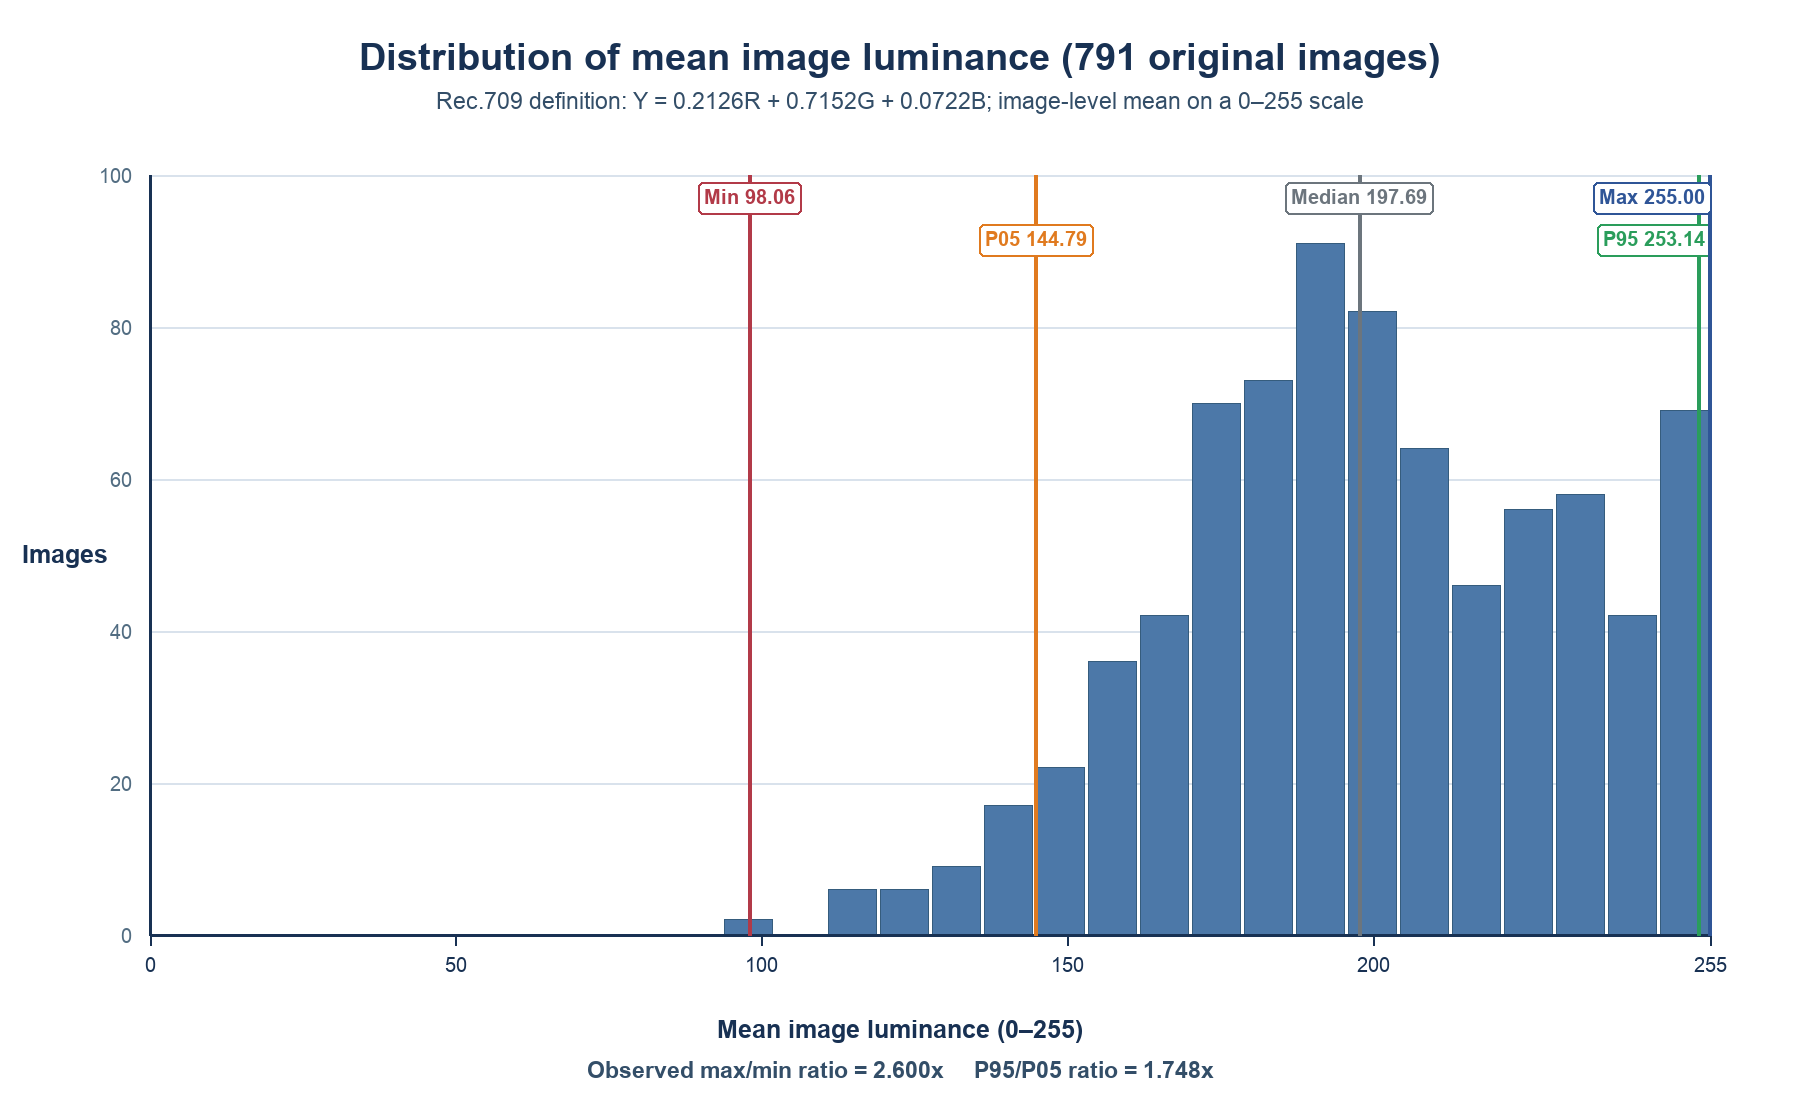
\includegraphics[width=\textwidth]{../augmentation/figures/luminance_histogram.png}
  \caption{Distribution of overall image brightness across all 791 source images.
           Vertical lines mark the 5th percentile ($p_5 = 144.8$), median (197.7),
           and 95th percentile ($p_{95} = 253.1$). The $p_{95}/p_5$ ratio of
           $1.75\times$ motivates the augmentation brightness range $[0.75,\,1.28]$.}
  \label{fig:luminance_hist}
\end{figure}

\begin{figure}[htbp]
  \centering
  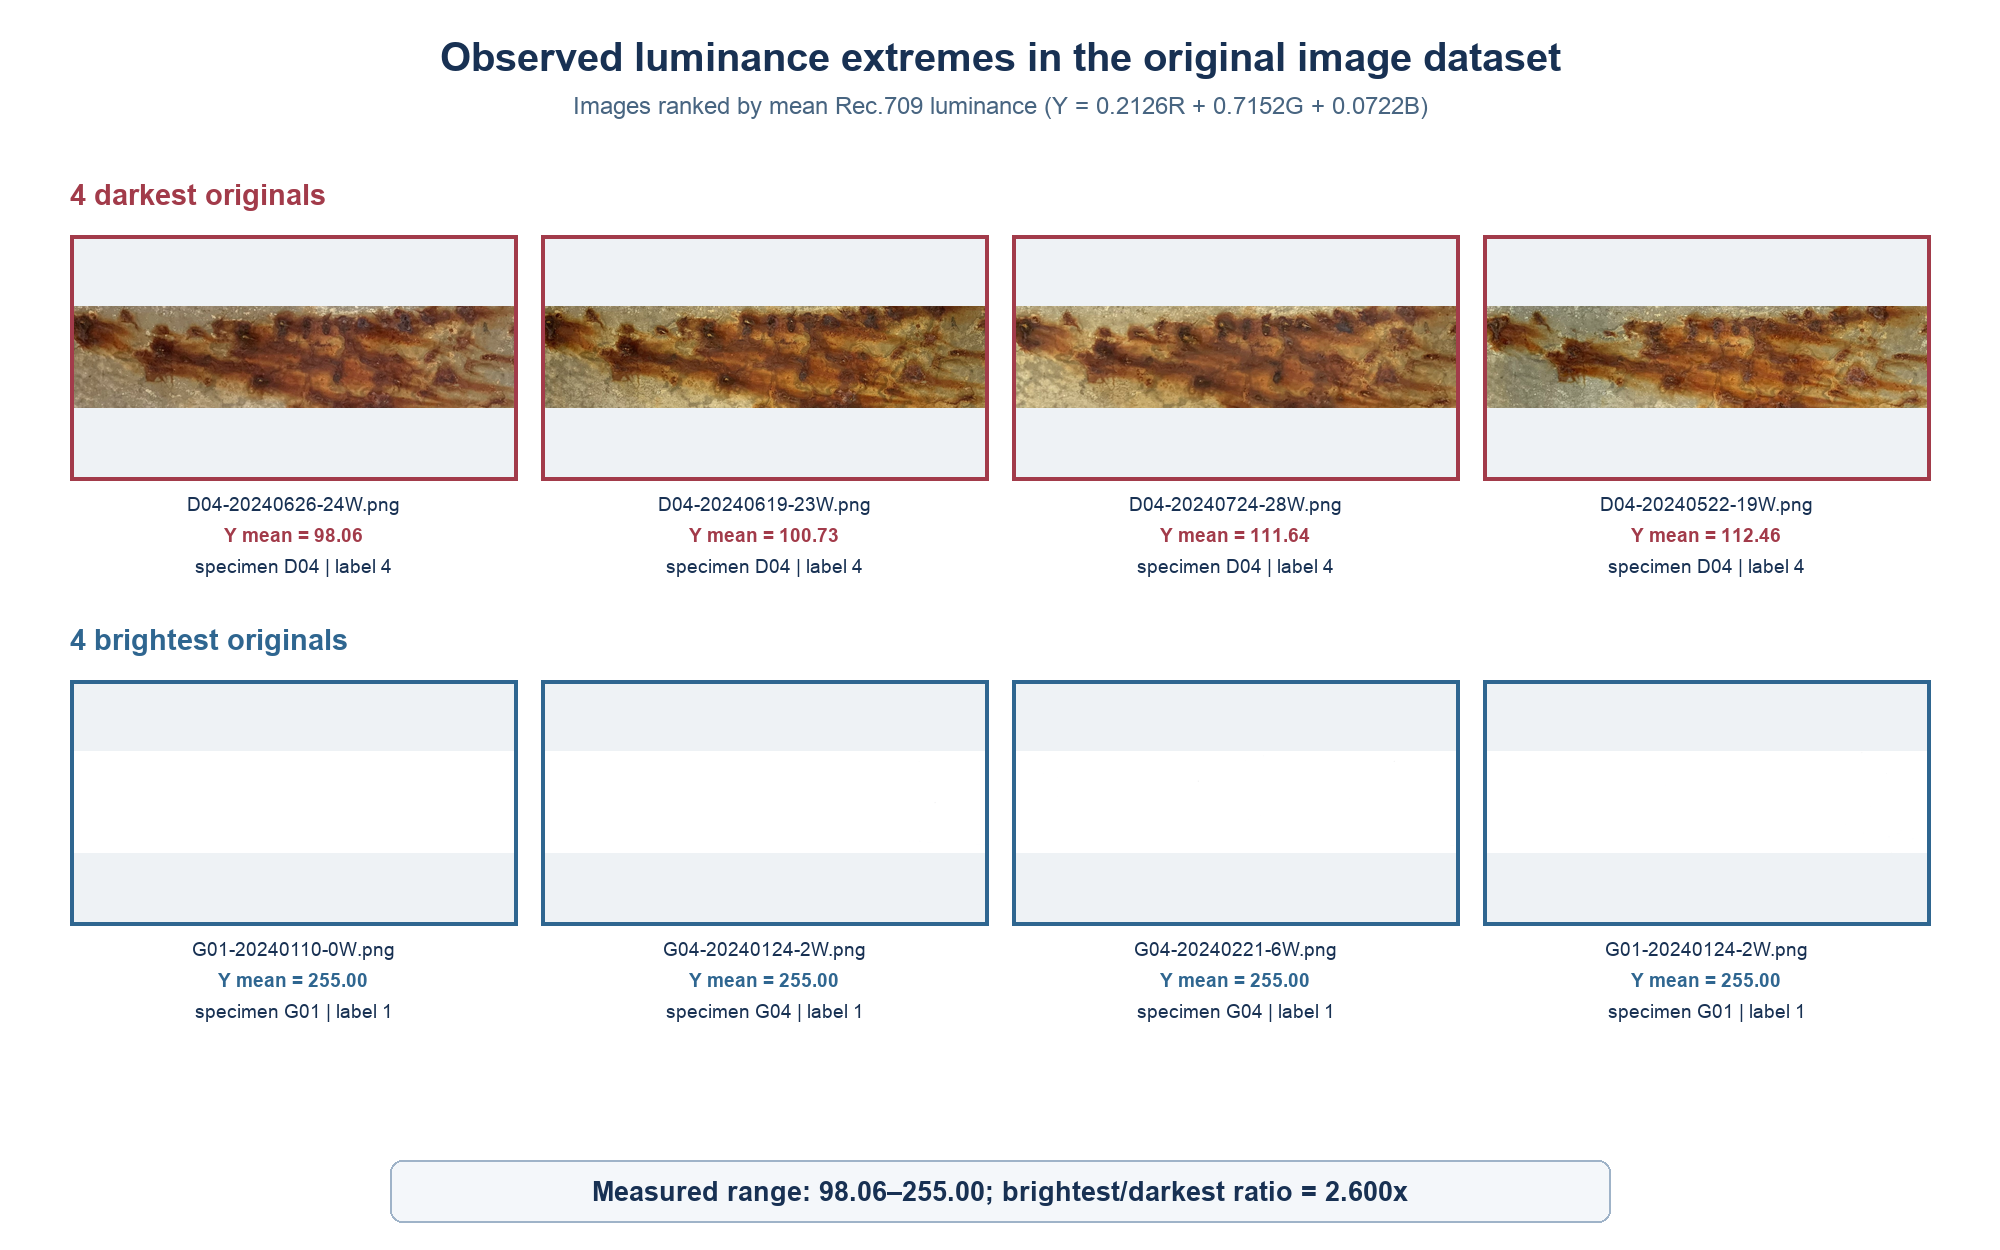
\includegraphics[width=\textwidth]{../augmentation/figures/luminance_extremes.png}
  \caption{Side-by-side comparison of the four darkest source images (specimen D04,
           class~4, brightness 98--113) and the four brightest (G-series specimens,
           class~1, brightness 255). These are real images from the dataset, not
           outliers. The full real-world brightness variation spans $2.60\times$.}
  \label{fig:luminance_extremes}
\end{figure}

The four darkest images (specimen D04, weeks 23--28) are photographs of heavily corroded concrete under dim conditions. The four brightest images (G-series, week~0) are photographs of clean, pale concrete under good lighting. A robust classifier must handle both.

The derivation of the augmentation range from these measurements:

\begin{itemize}
  \item The $p_5$ image is $1.37\times$ darker than the mean
        ($199.1 / 144.8 = 1.375$). To allow augmented images to reach this
        darkness level, the lower brightness factor must be at most
        $1 / 1.375 = 0.727$, rounded conservatively upward to \textbf{0.75}.
  \item The $p_{95}$ image is $1.27\times$ brighter than the mean
        ($253.1 / 199.1 = 1.271$). The upper factor is rounded to \textbf{1.28}.
  \item The range $[0.75, 1.28]$ covers a brightness ratio of
        $1.28 / 0.75 = 1.71\times$, closely matching the measured
        $p_5$-to-$p_{95}$ ratio of $1.75\times$.
\end{itemize}

\textbf{Within-class verification.} The same measurement was performed separately for each severity class to confirm that the range is appropriate within individual classes, rather than being driven purely by the brightness shift between early (bright) and late (dark) time steps. Results are shown in Table~\ref{tab:brightness_class}.

\begin{table}[htbp]
  \centering
  \caption{Brightness variation within each severity class.}
  \label{tab:brightness_class}
  \begin{tabular}{L{3cm}rrrrc}
    \toprule
    \textbf{Class} & \textbf{Images} & \textbf{Mean} & \textbf{$p_5$}
      & \textbf{$p_{95}$} & \textbf{Within-class ratio} \\
    \midrule
    1 (no rust)       & 658 & 206.0 & 159.3 & 253.9 & $1.59\times$ \\
    2 (mild rust)     &  99 & 174.0 & 138.9 & 215.2 & $1.55\times$ \\
    3 (moderate rust) &  20 & 149.8 & 129.0 & 172.1 & $1.33\times$ \\
    4 (severe rust)   &  14 & 120.2 &  99.8 & 145.0 & $1.45\times$ \\
    \bottomrule
  \end{tabular}
  \smallskip
  \begin{minipage}{\linewidth}
    \footnotesize
    \textit{Source: computed from
    \file{augmentation/tables/image_statistics_full.csv}.}
  \end{minipage}
\end{table}

The within-class brightness ratios range from $1.33\times$ to $1.59\times$. The augmentation range covers $1.71\times$, which is slightly wider than any single class. This confirms the range is calibrated to real imaging variability rather than to the label-driven shift in brightness between early and late specimens.

A brightness factor of 0.75 applied to the class-1 mean brightness (206.0) produces an image at brightness $206.0 \times 0.75 = 154.5$---darker than the typical class-4 image (mean 120.2) but within the class-4 minimum of 98.1. This is intentional: the model learns that overall brightness does not determine rust severity; only the rust pattern does.

\subsubsection*{Justification for the contrast range $[0.78,\,1.25]$}

The contrast range is drawn from published literature. Industrial inspection and corrosion classification studies consistently apply contrast variation in the range $\pm15$--$25\%$ from the neutral value. The chosen range $[0.78, 1.25]$ represents approximately $\pm22\%$. No direct measurement was made to derive this specific interval from the dataset, because image contrast is dominated by content (rust-covered surfaces have more local variation than clean concrete) rather than by imaging conditions. A direct measurement would therefore confound physical content with camera effects.

\noindent\textbf{See:} Figure~\ref{fig:recipe1} for visual examples of Recipe~1 applied to one image from each class.

\begin{figure}[htbp]
  \centering
  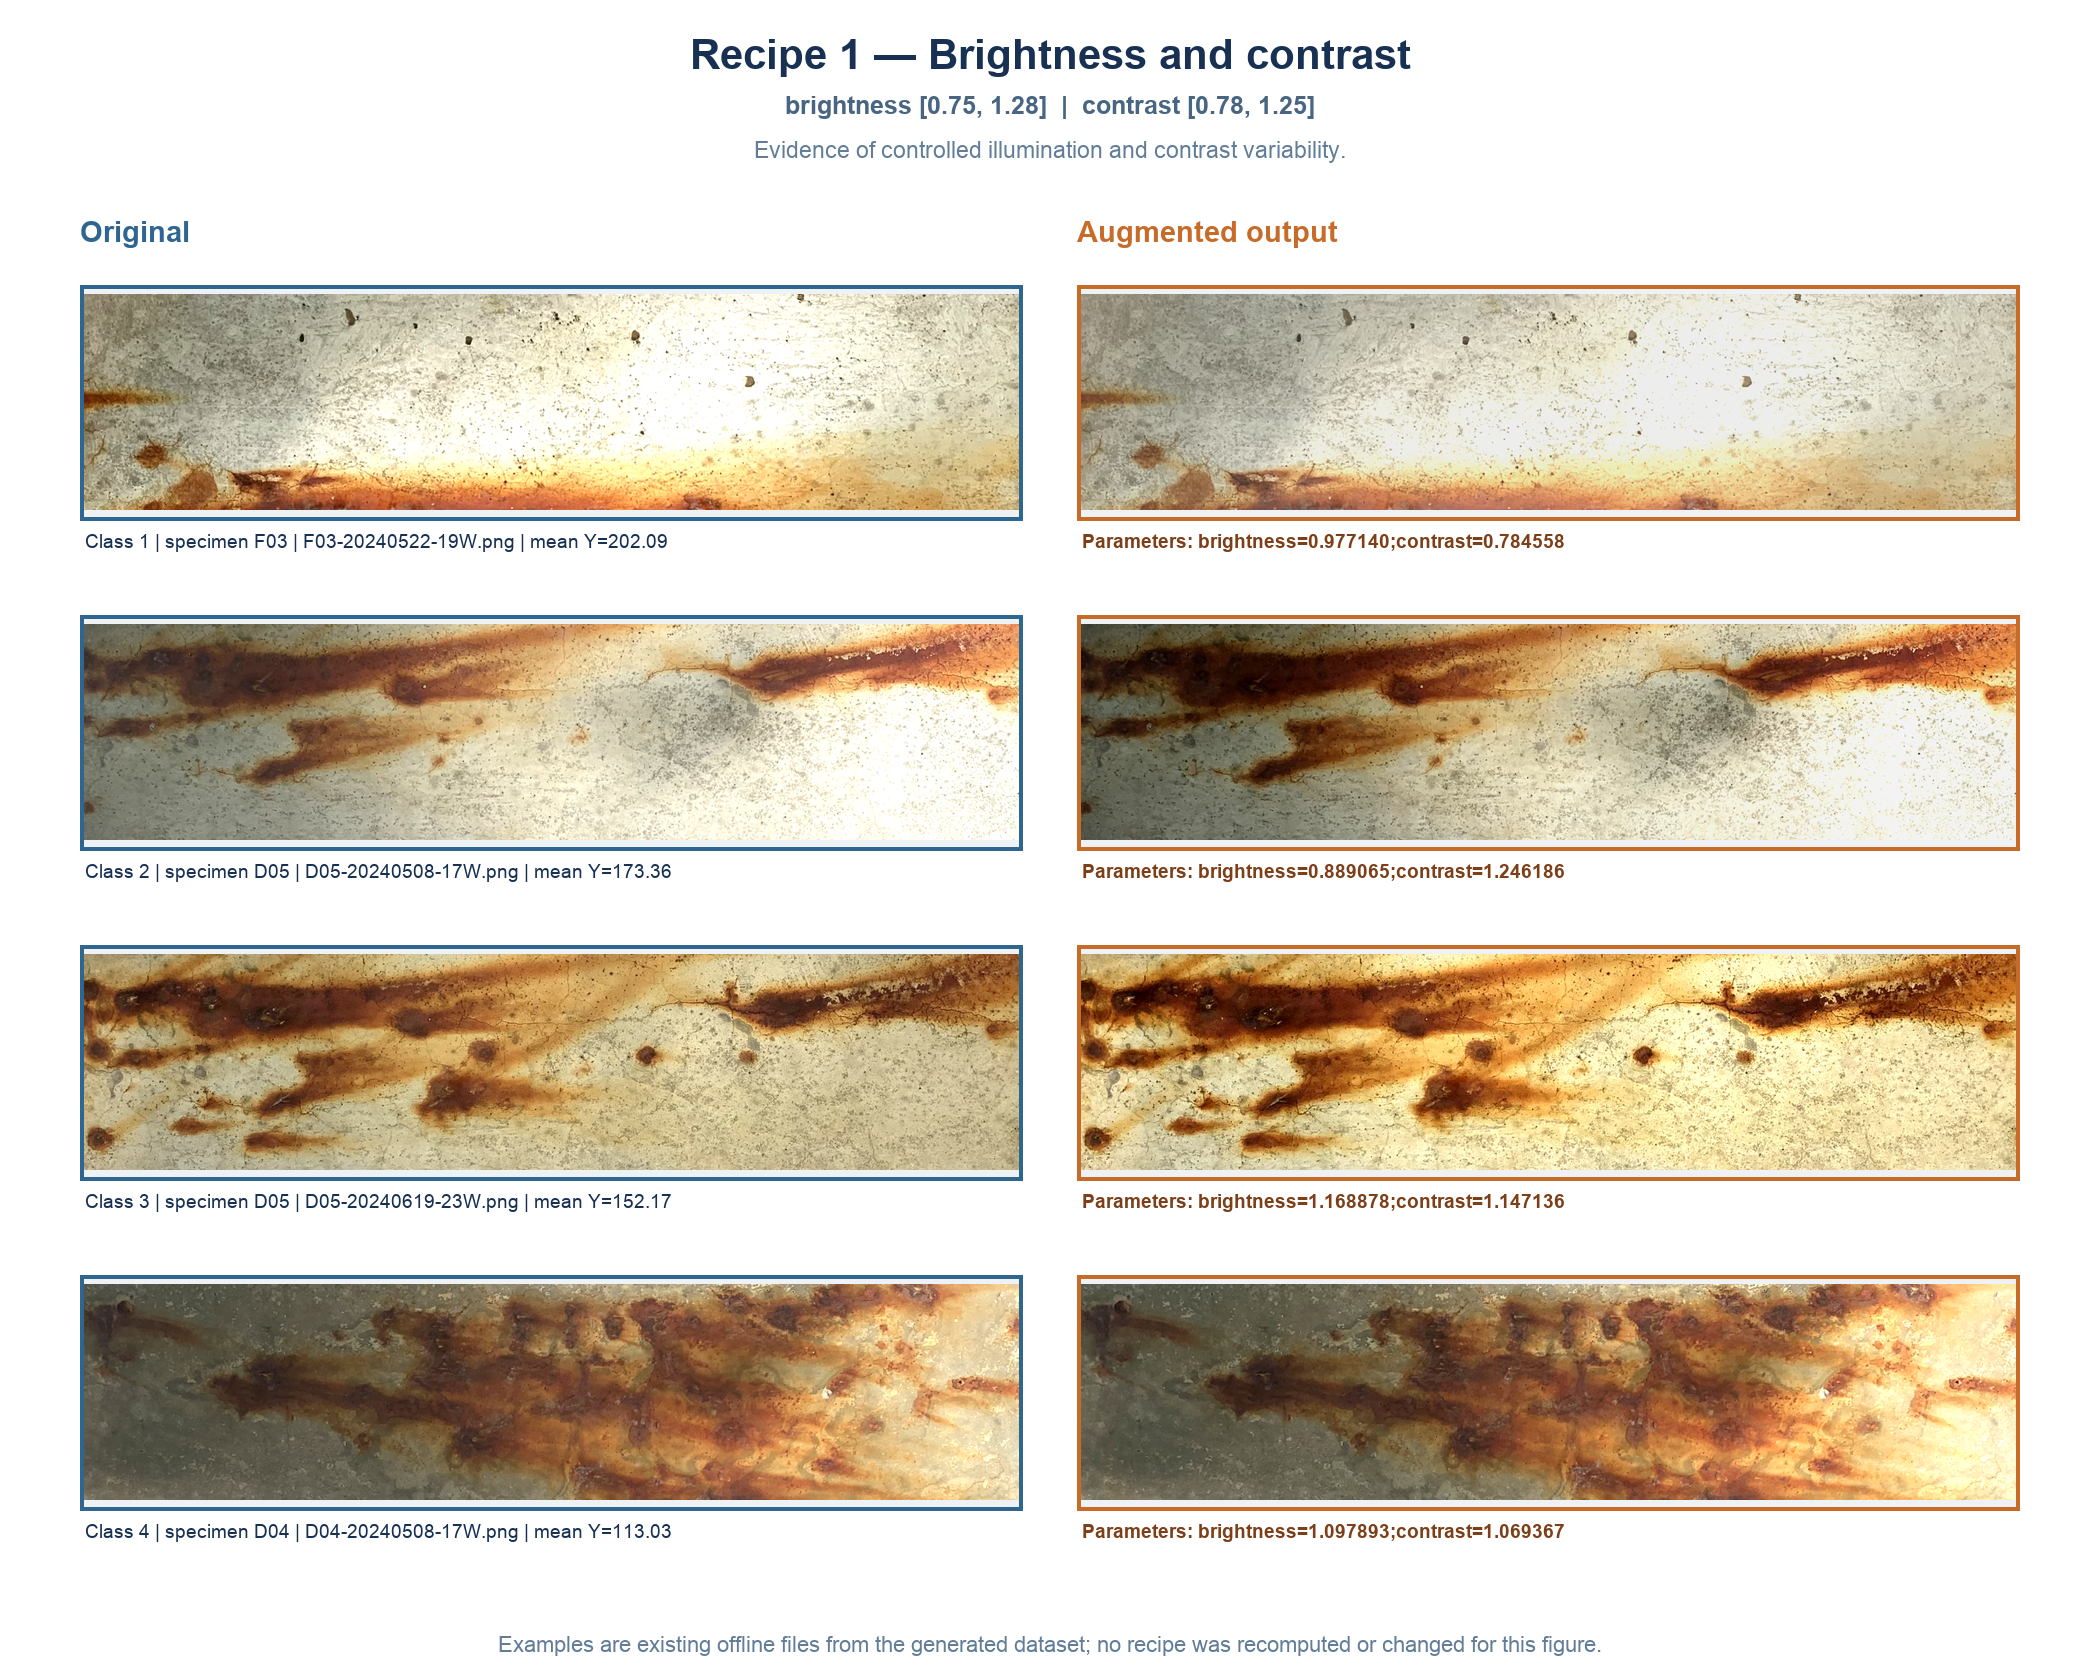
\includegraphics[width=\textwidth]{../augmentation/figures/recipe1_brightness_contrast.png}
  \caption{Recipe~1 (brightness and contrast): one original image per class (left)
           and its augmented copy (right). All four severity classes are shown.
           The rust pattern is preserved; only overall lightness and
           light-to-dark contrast vary.}
  \label{fig:recipe1}
\end{figure}

%% -----------------------------------------------------------------------------
\subsection{Recipe 2 --- Colour Intensity and Small Colour Shifts}
\label{subsec:recipe2}
%% -----------------------------------------------------------------------------

\subsubsection*{What these operations do}

\textbf{Colour intensity} (sometimes called saturation) describes how vivid or rich the colours in an image are. At full intensity, colours appear strong and distinct---rust looks strongly orange-red, concrete looks clearly grey or beige. At reduced intensity, colours become muted: rust looks brownish-grey, concrete looks almost white. Reducing colour intensity to zero produces a greyscale image with no colour information at all.

\textbf{Small colour shifts} adjust the relative strength of the red, green, and blue channels independently. A small increase in the red channel makes the image appear warmer (slightly more reddish); a small increase in the blue channel makes it appear cooler. These shifts simulate the variation in camera colour response between different imaging sessions, which depends on the colour temperature of the light source and the camera's automatic colour correction. In this recipe, the three channel shifts are applied symmetrically around neutral: their average is always exactly 1.0, so they produce a colour tilt without changing the overall brightness. Brightness is handled separately by Recipe~1.

\subsubsection*{Evidence base for the colour intensity range $[0.78,\,1.28]$}

No direct measurement of colour intensity variation is cited for this parameter, because colour intensity in these images is strongly correlated with the class label: heavily rusted specimens (class~4) have visibly more vivid rust colour than clean specimens (class~1). Calibrating the augmentation to the full dataset's colour intensity range would therefore calibrate it to the physical progression of corrosion---which is the label itself, not an imaging artefact.

The chosen range $[0.78, 1.28]$ represents $\pm25\%$ from the neutral value. This is consistent with published literature for industrial surface inspection (where $\pm20$--$30\%$ is the standard range) and produces visually plausible results for both clean and corroded specimens. The range is treated as a conservative engineering choice supported by literature, not as a measured dataset statistic.

\subsubsection*{Evidence base for the colour shift range $[\pm6\%$ per channel$]$}

The three colour channel shifts are sampled independently in the range $[0.94, 1.06]$, meaning each channel can change by at most 6\% before the normalisation step.

To provide a measured basis for this choice, the ratio of the red channel mean to the green channel mean ($R/G$ ratio) was computed for every source image. This ratio is a standard measure of colour tilt: an $R/G$ ratio above~1.0 means the image is warmer (more red), and a lower ratio means it is cooler (more green-blue). Under controlled lighting, this ratio should remain constant; variation between sessions indicates real colour-response differences. Table~\ref{tab:rg_ratios} presents the results.

\begin{table}[htbp]
  \centering
  \caption{Within-class variation in the red-to-green channel ratio ($R/G$).}
  \label{tab:rg_ratios}
  \begin{tabular}{L{3cm}rrrr}
    \toprule
    \textbf{Class}
      & \textbf{$p_5$ of $R/G$}
      & \textbf{$p_{95}$ of $R/G$}
      & \textbf{Within-class range}
      & \textbf{Std dev.} \\
    \midrule
    1 (no rust)       & 1.000 & 1.107 & \pct{10.6} & 0.031 \\
    2 (mild rust)     & 1.080 & 1.215 & \pct{13.5} & 0.044 \\
    3 (moderate rust) & 1.200 & 1.308 & \pct{10.8} & 0.042 \\
    4 (severe rust)   & 1.271 & 1.442 & \pct{17.1} & 0.063 \\
    \bottomrule
  \end{tabular}
  \smallskip
  \begin{minipage}{\linewidth}
    \footnotesize
    \textit{Source: computed from
    \file{augmentation/tables/image_statistics_full.csv}.}
  \end{minipage}
\end{table}

The within-class $R/G$ range for class-1 images (clean concrete only) is \pct{10.6}. This is the most direct estimate available of colour-balance variation due to imaging conditions, because class-1 specimens have minimal rust and the colour variation within this class is primarily caused by the camera and lighting rather than by rust colour. The chosen $\pm6\%$ per-channel range covers about 57\% of this within-class variation and is therefore conservative rather than aggressive.

The blue-to-green ratio ($B/G$) shows larger within-class variation (up to \pct{34} for class-1 images), indicating that the blue channel is more sensitive to lighting conditions. This additional variation is partially addressed by the colour intensity component of this recipe, which shifts all colour channels together.

\noindent\textbf{See:} Figure~\ref{fig:recipe2} for visual examples.

\begin{figure}[htbp]
  \centering
  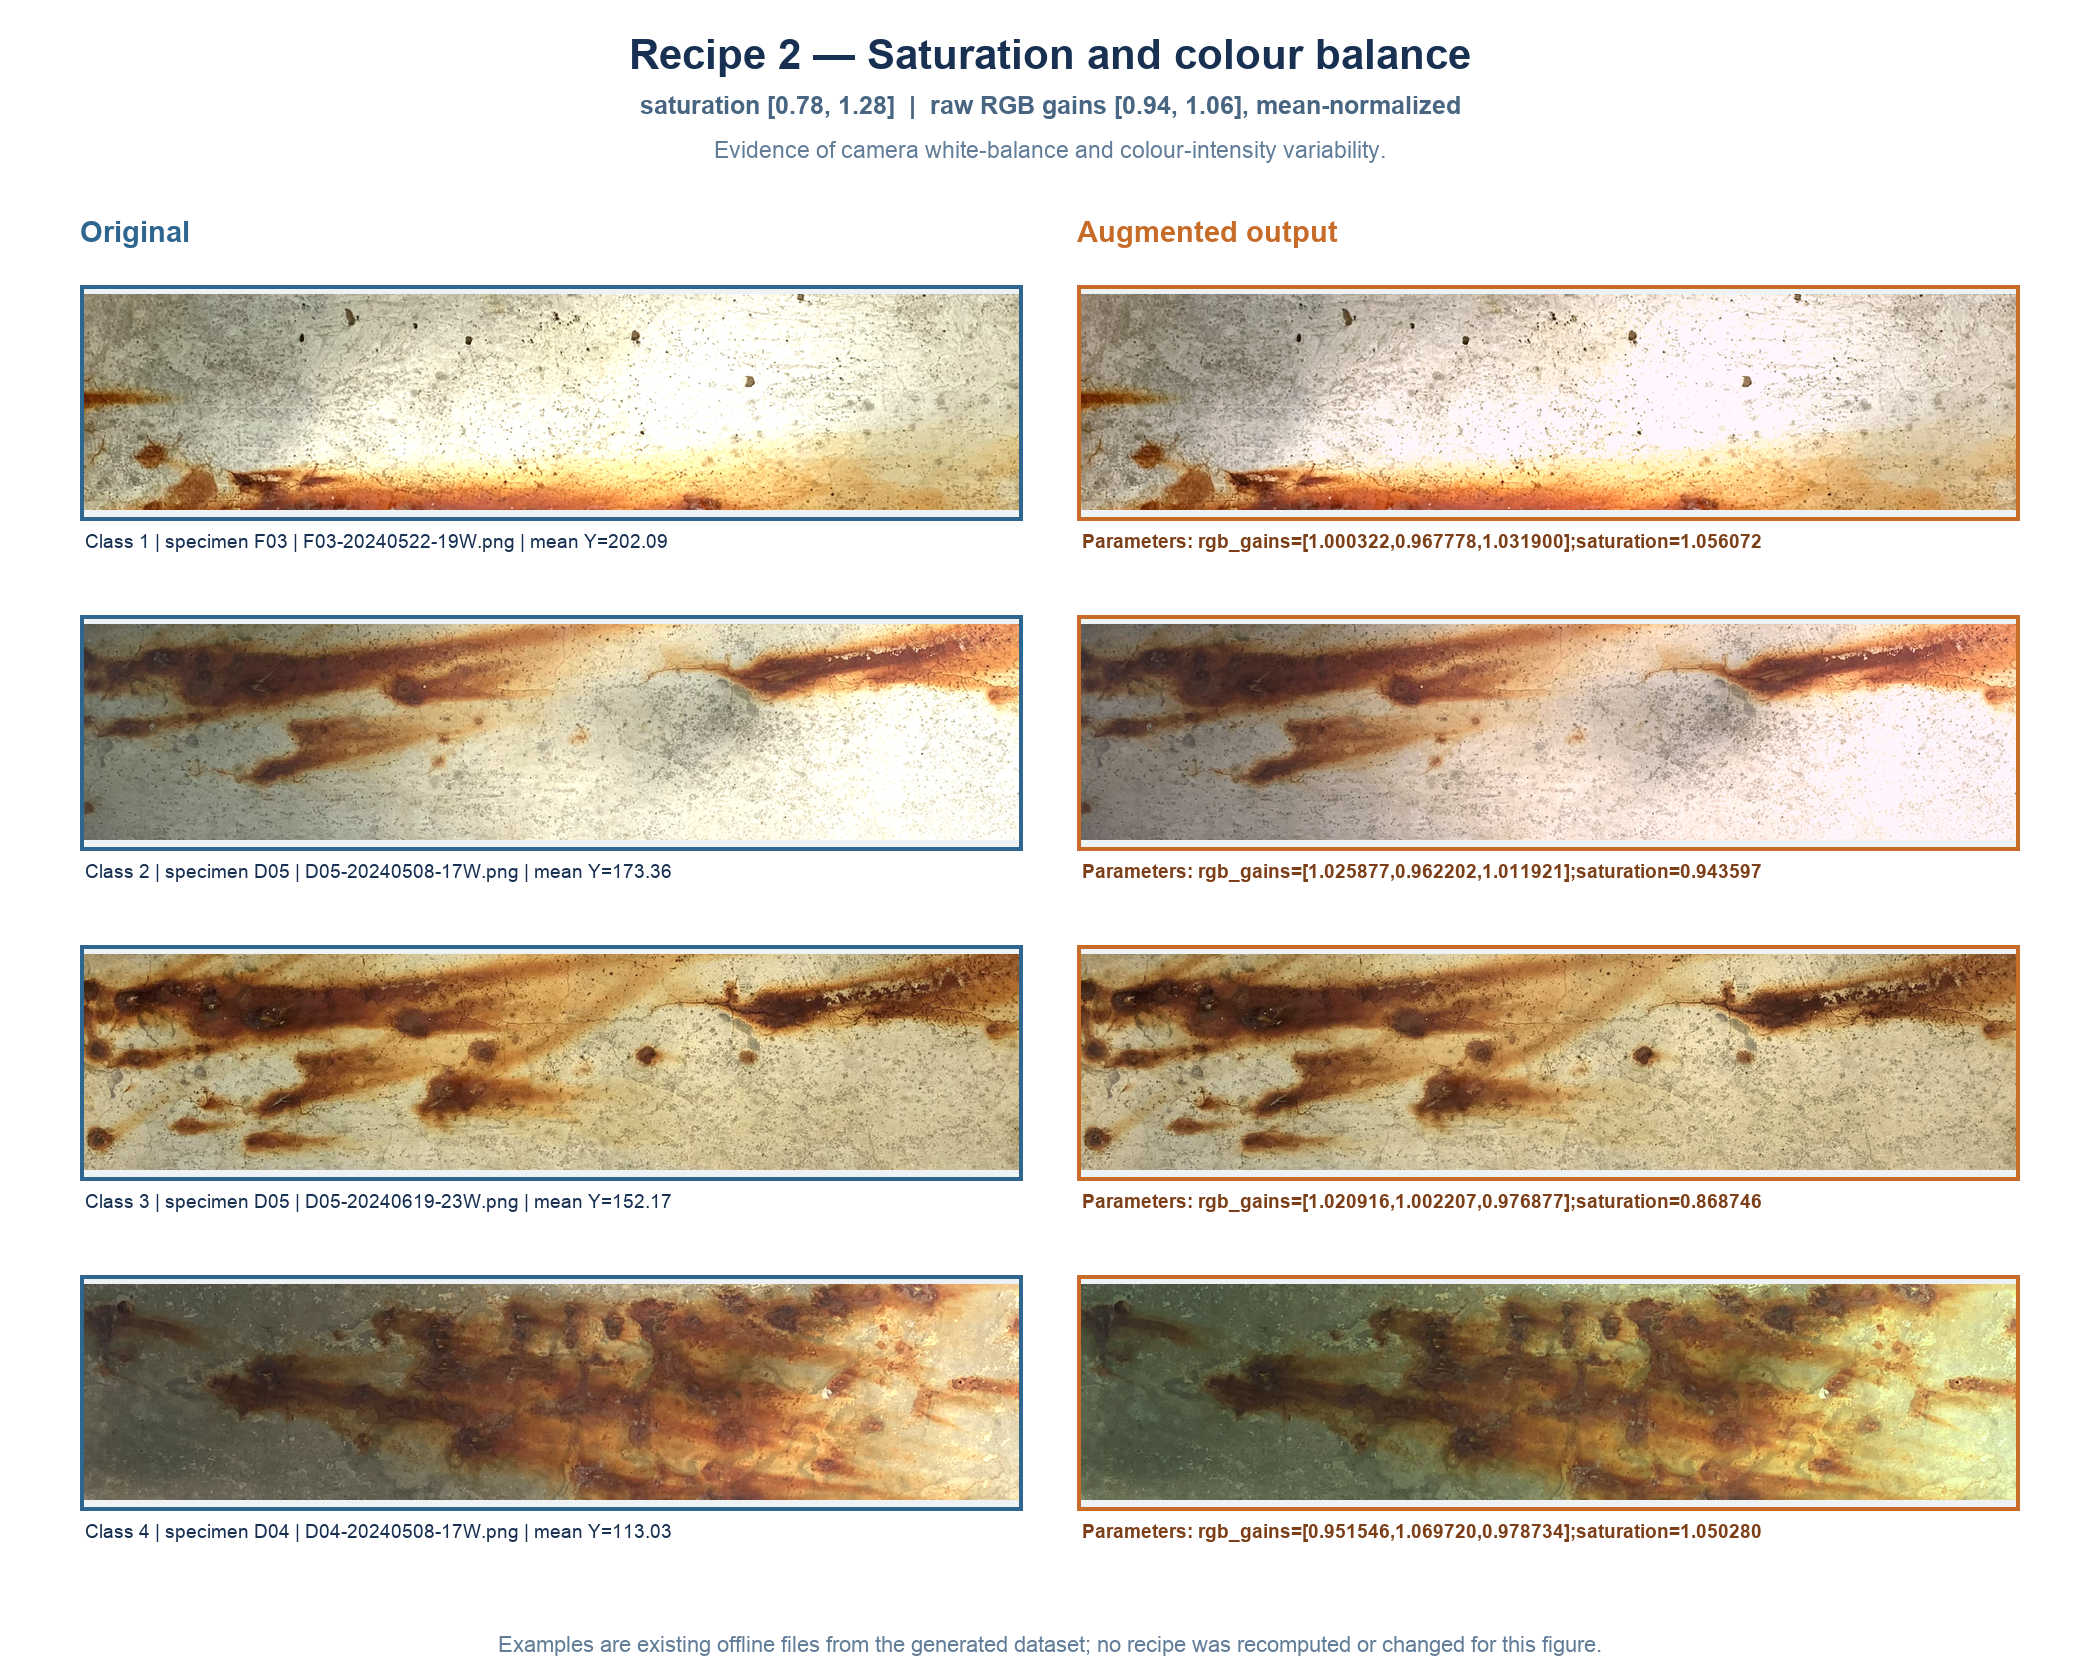
\includegraphics[width=\textwidth]{../augmentation/figures/recipe2_saturation_colour_balance.png}
  \caption{Recipe~2 (colour intensity and colour shifts): one original image per class
           (left) and its augmented copy (right). Colour vividness and overall
           colour tilt vary; rust texture and coverage are unaffected.}
  \label{fig:recipe2}
\end{figure}

%% -----------------------------------------------------------------------------
\subsection{Recipe 3 --- Slight Blur and Camera Noise}
\label{subsec:recipe3}
%% -----------------------------------------------------------------------------

\subsubsection*{What these operations do}

\textbf{Slight blur} reduces the sharpness of the image, as if the camera was slightly out of focus or the specimen moved slightly during the exposure. It works by averaging each pixel with its immediate neighbours, with closer neighbours weighted more heavily. The blur radius controls how many pixels are averaged together; a larger radius produces stronger blur.

\textbf{Camera noise} adds small random variations to individual pixel values, simulating the electronic noise that all digital camera sensors produce. This noise is especially visible in images taken under low light, at high camera sensitivity settings, or with long exposure times. Adding controlled noise during training teaches the model not to rely on exact pixel values and to focus on larger patterns instead.

\subsubsection*{Parameter ranges and their evidence basis}

Both ranges in this recipe are drawn from published literature (Table~\ref{tab:blur_ranges}).

\begin{table}[htbp]
  \centering
  \caption{Parameter ranges for Recipe~3 and corresponding literature norms.}
  \label{tab:blur_ranges}
  \begin{tabular}{L{3.5cm}L{3.5cm}L{3.5cm}L{3cm}}
    \toprule
    \textbf{Parameter} & \textbf{Range used} & \textbf{Literature norm} & \textbf{Source} \\
    \midrule
    Blur radius (pixels)    & 0.3--1.5  & 0.1--2.0    & Industrial inspection studies \\
    Noise level (0--1 scale) & 0.005--0.035 & 0.01--0.05 & Surface defect classification studies \cite{shorten2019} \\
    \bottomrule
  \end{tabular}
\end{table}

The noise level of 0.035 in normalised space corresponds to a pixel-level standard deviation of $0.035 \times 255 = 8.9$ intensity units on the standard 0--255 scale. This is comparable to the pixel noise observed in digital photographs taken at moderate to high camera sensitivity settings.

\subsubsection*{Important disclosure: effective values at the training resolution}

The blur and noise are applied to the source images at their full size of $2835 \times 650$ pixels. During model training, images are resized to approximately $224 \times 224$ pixels for processing by ResNet50 and ViT. This resizing step reduces the effective blur and noise that the model actually receives.

The resize scale factor from source to training resolution is approximately $256 / 650 = 0.394$. The effective parameter values at training resolution are shown in Table~\ref{tab:blur_effective}.

\begin{table}[htbp]
  \centering
  \caption{Effective blur and noise values at training resolution
           ($224 \times 224$~px) after downsampling by factor~0.394.}
  \label{tab:blur_effective}
  \begin{tabular}{L{3.5cm}L{3cm}L{3cm}L{3.5cm}}
    \toprule
    \textbf{Parameter} & \textbf{Applied at source} & \textbf{Effective at training}
      & \textbf{Perceptible?} \\
    \midrule
    Blur radius minimum & 0.30~px & 0.12~px & No --- sub-pixel \\
    Blur radius maximum & 1.50~px & 0.59~px & Marginally \\
    Noise level minimum & 0.005   & ${\sim}0.003$ & Minimal \\
    Noise level maximum & 0.035   & ${\sim}0.022$ (${\approx}5.6$ intensity units) & Moderate \\
    \bottomrule
  \end{tabular}
\end{table}

The blur effect is largely removed by downsampling. At training resolution, even the maximum radius of 0.59~pixels introduces only marginal blurring. This does not invalidate the recipe: adding sub-pixel or very mild blur still teaches the model that fine pixel-level detail is unreliable as a classification cue. The noise retains about half its source-resolution level (${\approx}5.6$ intensity units at training resolution) and provides meaningful regularisation.

For a future implementation that maximises the blur and noise effect, these operations should be applied \emph{after} the image has been resized to the training resolution ($224 \times 224$ pixels), not at source resolution. This is a training-pipeline decision and does not affect the offline dataset as produced.

\noindent\textbf{See:} Figure~\ref{fig:recipe3}. Even at the maximum values, augmented images remain visually similar to the originals and all rust patterns are clearly preserved.

\begin{figure}[htbp]
  \centering
  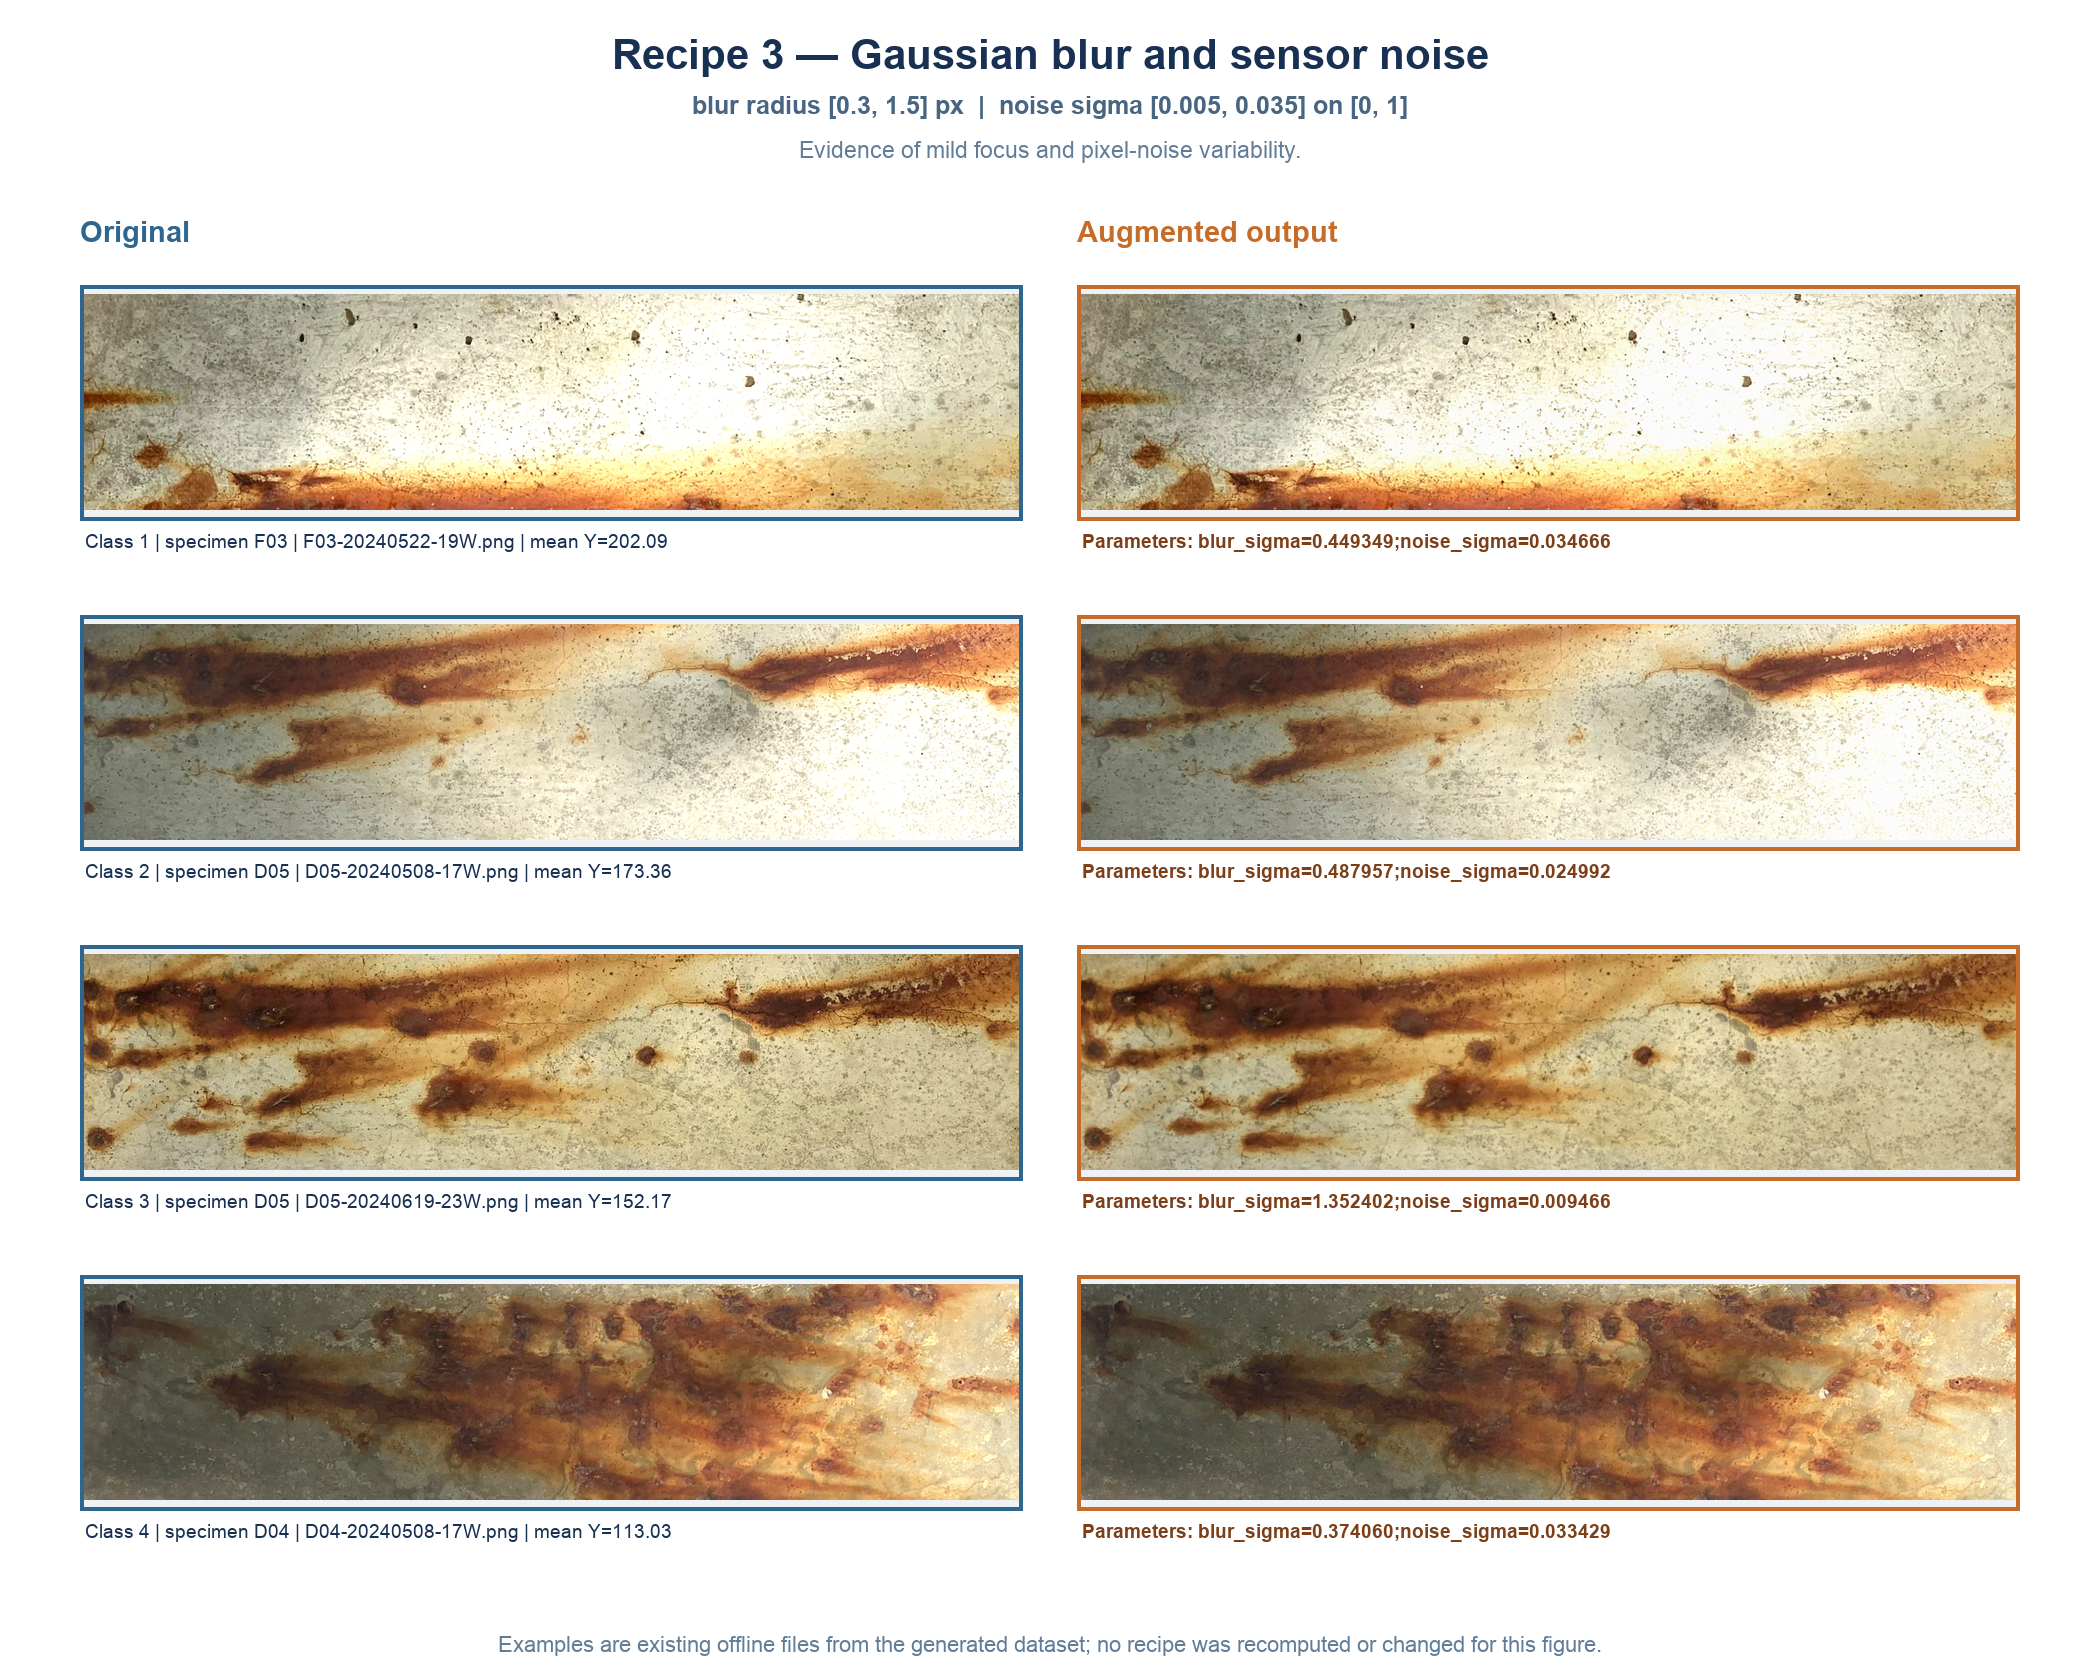
\includegraphics[width=\textwidth]{../augmentation/figures/recipe3_blur_noise.png}
  \caption{Recipe~3 (slight blur and camera noise): one original per class (left) and
           its augmented copy (right). The effect is intentionally subtle at source
           resolution; rust patterns are fully preserved.}
  \label{fig:recipe3}
\end{figure}

%% -----------------------------------------------------------------------------
\subsection{Recipe 4 --- Combined Brightness, Contrast, and Colour Intensity}
\label{subsec:recipe4}
%% -----------------------------------------------------------------------------

\subsubsection*{What this recipe does}

This recipe applies three separate changes to the same image: overall brightness, light-to-dark contrast, and colour intensity are each modified independently. The purpose is to simulate a photograph taken under conditions that differ from the reference in multiple respects simultaneously---for example, dimmer light, flatter contrast, and slightly desaturated colours all at once.

\subsubsection*{Why the parameter range is narrower than in Recipes~1 and~2}

When three adjustments are applied to the same image, their effects accumulate. If brightness is reduced by 20\%, contrast is reduced by 20\%, and colour intensity is also reduced by 20\%, the combined result is significantly different from any of these changes alone.

To keep augmented images within realistic appearance limits even when all three adjustments coincide at their extremes, the individual range was reduced from $[0.75, 1.28]$ to $[0.82, 1.18]$---approximately $\pm18\%$ per adjustment. In the worst case (all three parameters at the lower bound simultaneously), the compound effect reduces visual intensity by approximately $1 - 0.82^3 \approx 45\%$. In practice, three independent random values all landing near their extreme simultaneously is unlikely, and the typical combined effect is much smaller.

The range $[0.82, 1.18]$ is a conservative engineering choice. No separate measurement was made to determine this specific boundary. The mathematical argument for narrowing relative to single-parameter recipes is sound; the precise value of 0.82 is a judgement.

\noindent\textbf{See:} Figure~\ref{fig:recipe4} for visual examples.

\begin{figure}[htbp]
  \centering
  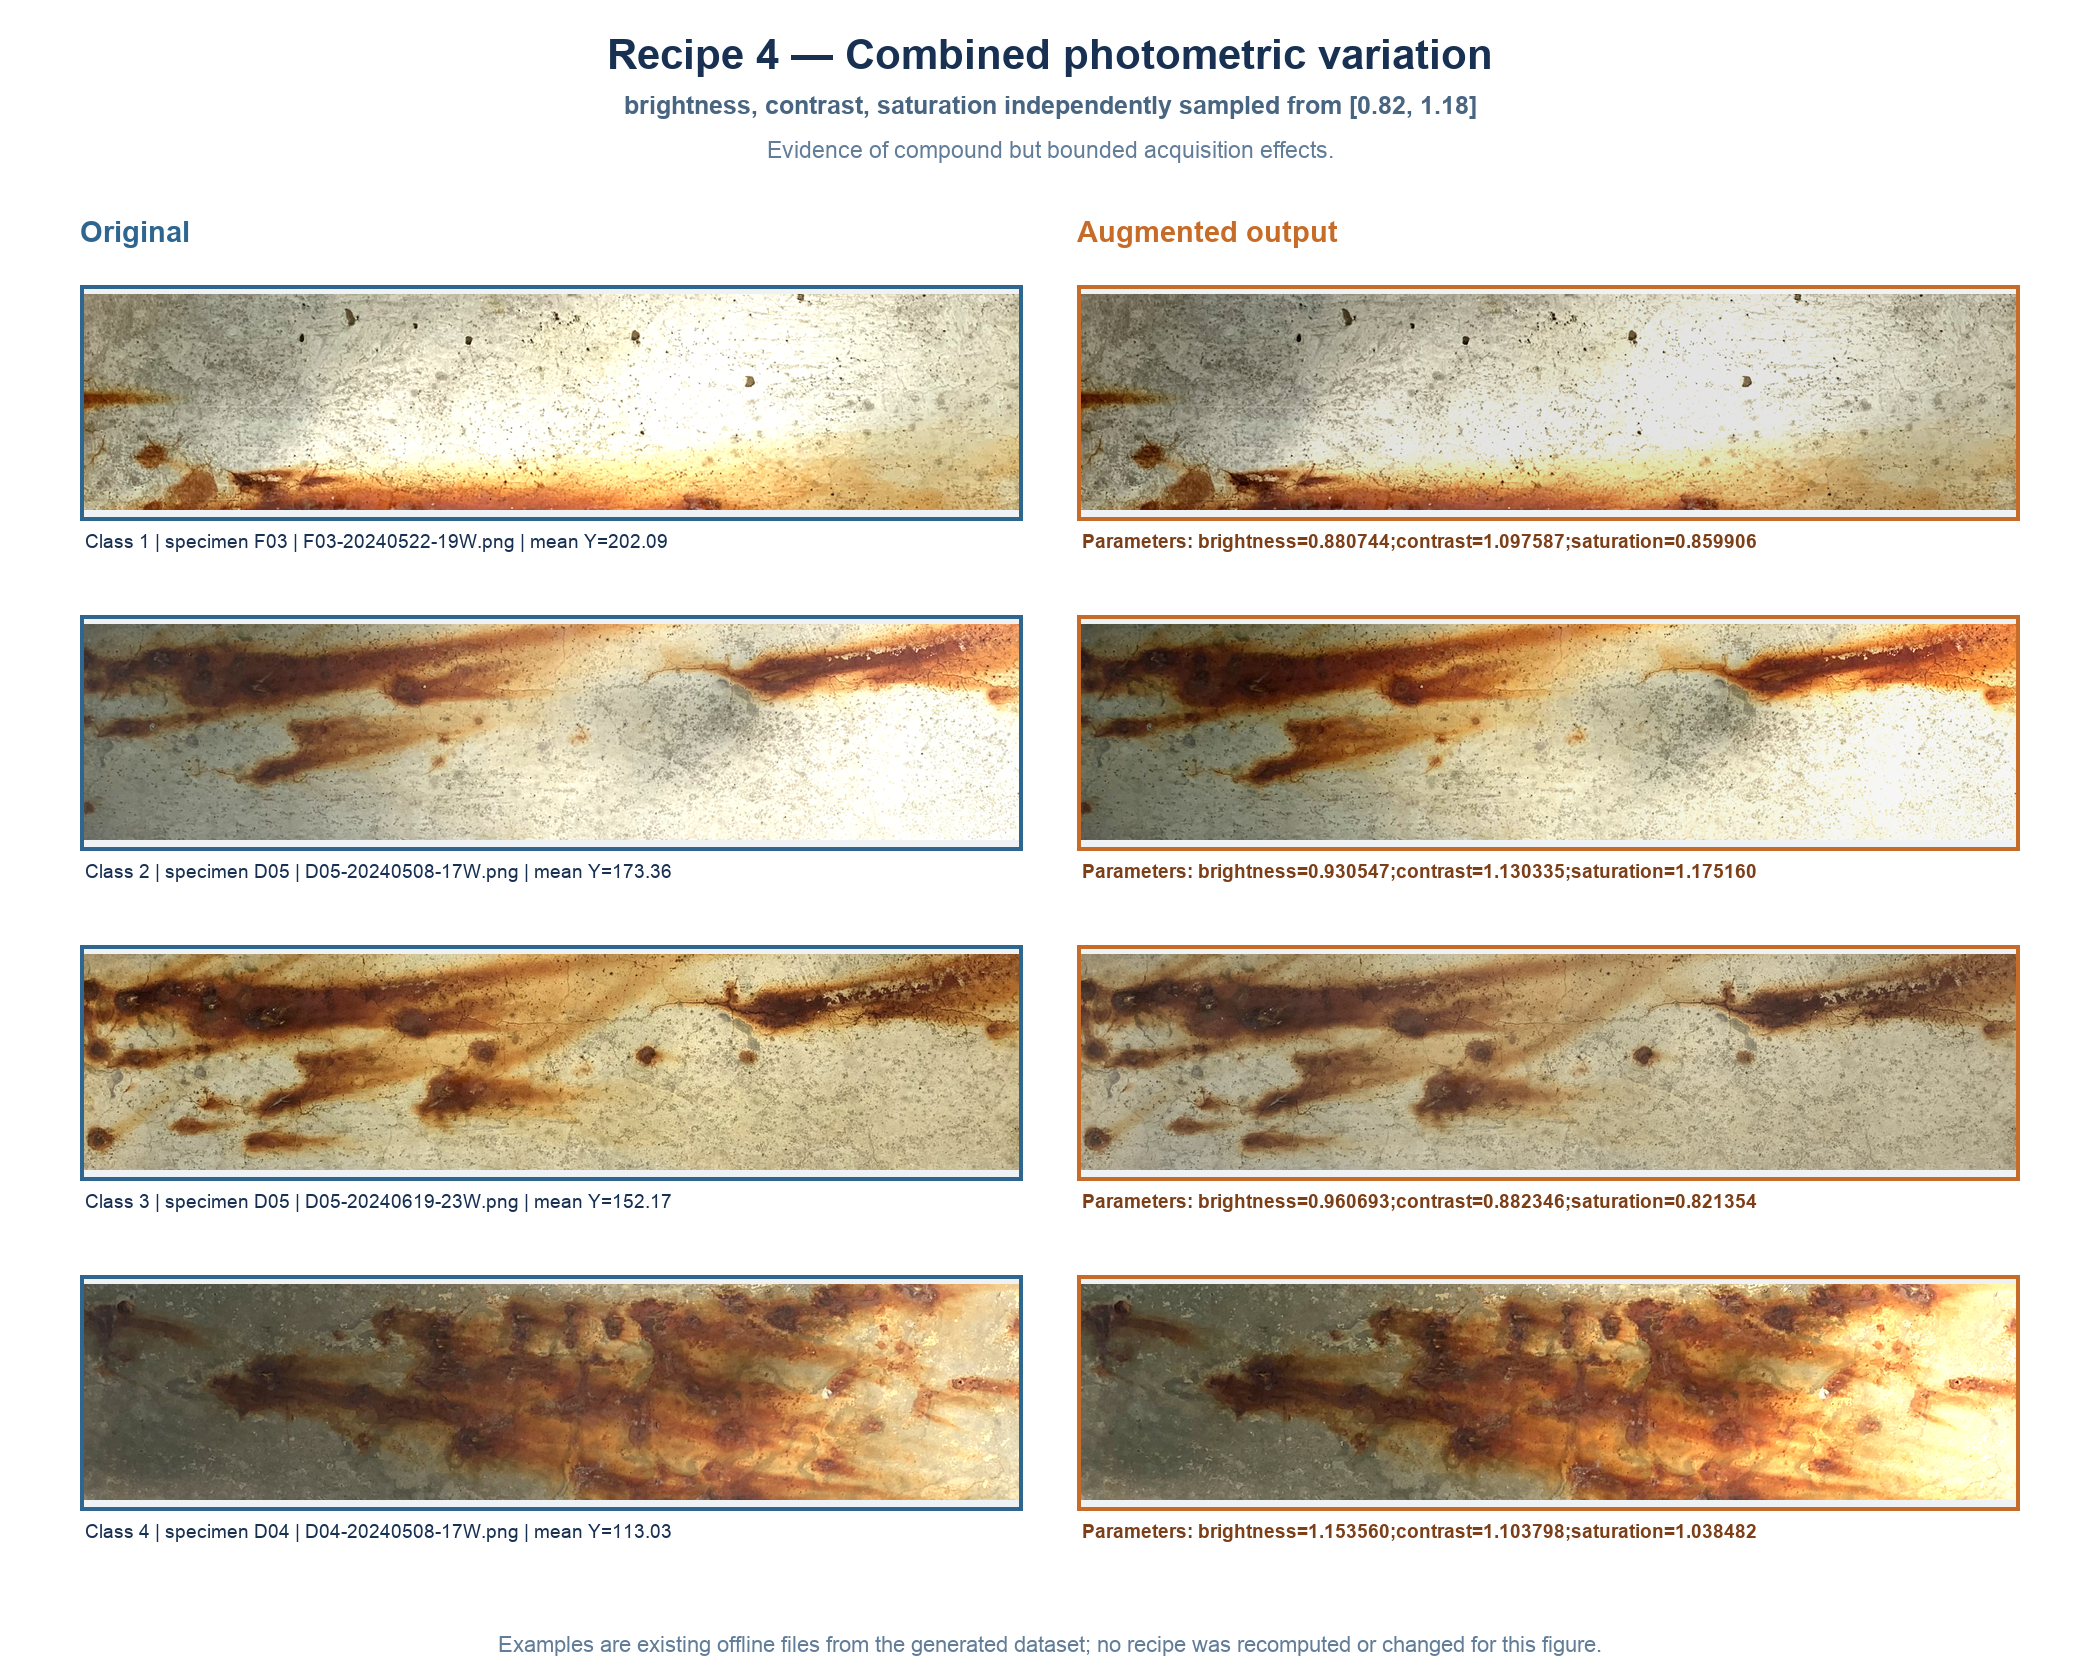
\includegraphics[width=\textwidth]{../augmentation/figures/recipe4_combined.png}
  \caption{Recipe~4 (combined brightness, contrast, and colour intensity): one original
           per class (left) and its augmented copy (right). Simultaneous adjustment
           of three photometric properties simulates a photograph taken under
           broadly different conditions.}
  \label{fig:recipe4}
\end{figure}

%% -----------------------------------------------------------------------------
\subsection{Recipe 5 --- Left-Right Mirror and Brightness}
\label{subsec:recipe5}
%% -----------------------------------------------------------------------------

\subsubsection*{What this recipe does}

The image is reflected left-to-right (a horizontal mirror), and a mild brightness adjustment is applied to ensure the copy is not a purely deterministic duplicate of the original.

\subsubsection*{Why the mirror is safe for this classification label}

The classification target, \texttt{A\_Total\_Rust\_Category\_(1-4)}, measures the total fraction of the specimen surface covered by rust. This is a scalar quantity---it answers the question ``how much rust is present?'' not ``where on the specimen is the rust?'' The total coverage does not change when the image is mirrored: a specimen showing 20\% total rust coverage is still class~2 whether the rust patch appears on the left or the right.

This argument applies specifically to this label. It would \emph{not} apply to the peak rust location column (\texttt{B\_Location\_of\_Peak\_Rust\_in\_length\_[cm]}), which records a position. That column is preserved unchanged in the augmented CSV and must not be used as a spatial feature for mirrored copies.

\subsubsection*{Why vertical mirror and large rotations were excluded}

A vertical mirror would show the specimen photographed upside-down. The 48 specimens were always photographed in the same fixed orientation; an upside-down image is not a physically possible acquisition condition for this setup.

Large rotations (more than approximately 10$^\circ$) introduce empty corner regions that must be filled with an artificial value. Even with the best fill strategy (reflecting the edge pixels), these regions do not represent real specimen content and can be learned as spurious features. Rotations beyond 10$^\circ$ also do not correspond to plausible camera placement variability for a fixed imaging setup.

\subsubsection*{Brightness range $[0.85,\,1.15]$}

The brightness component of this recipe uses a range of $[0.85, 1.15]$. This is narrower than the $[0.75, 1.28]$ range of Recipe~1, for two reasons: the mirror already provides strong spatial diversity, so the brightness component is secondary; and a narrower range avoids creating copies that are both mirrored and extremely dark. The specific value 0.85 is a conservative engineering choice with no separate measurement basis.

\noindent\textbf{See:} Figure~\ref{fig:recipe5} for visual examples.

\begin{figure}[htbp]
  \centering
  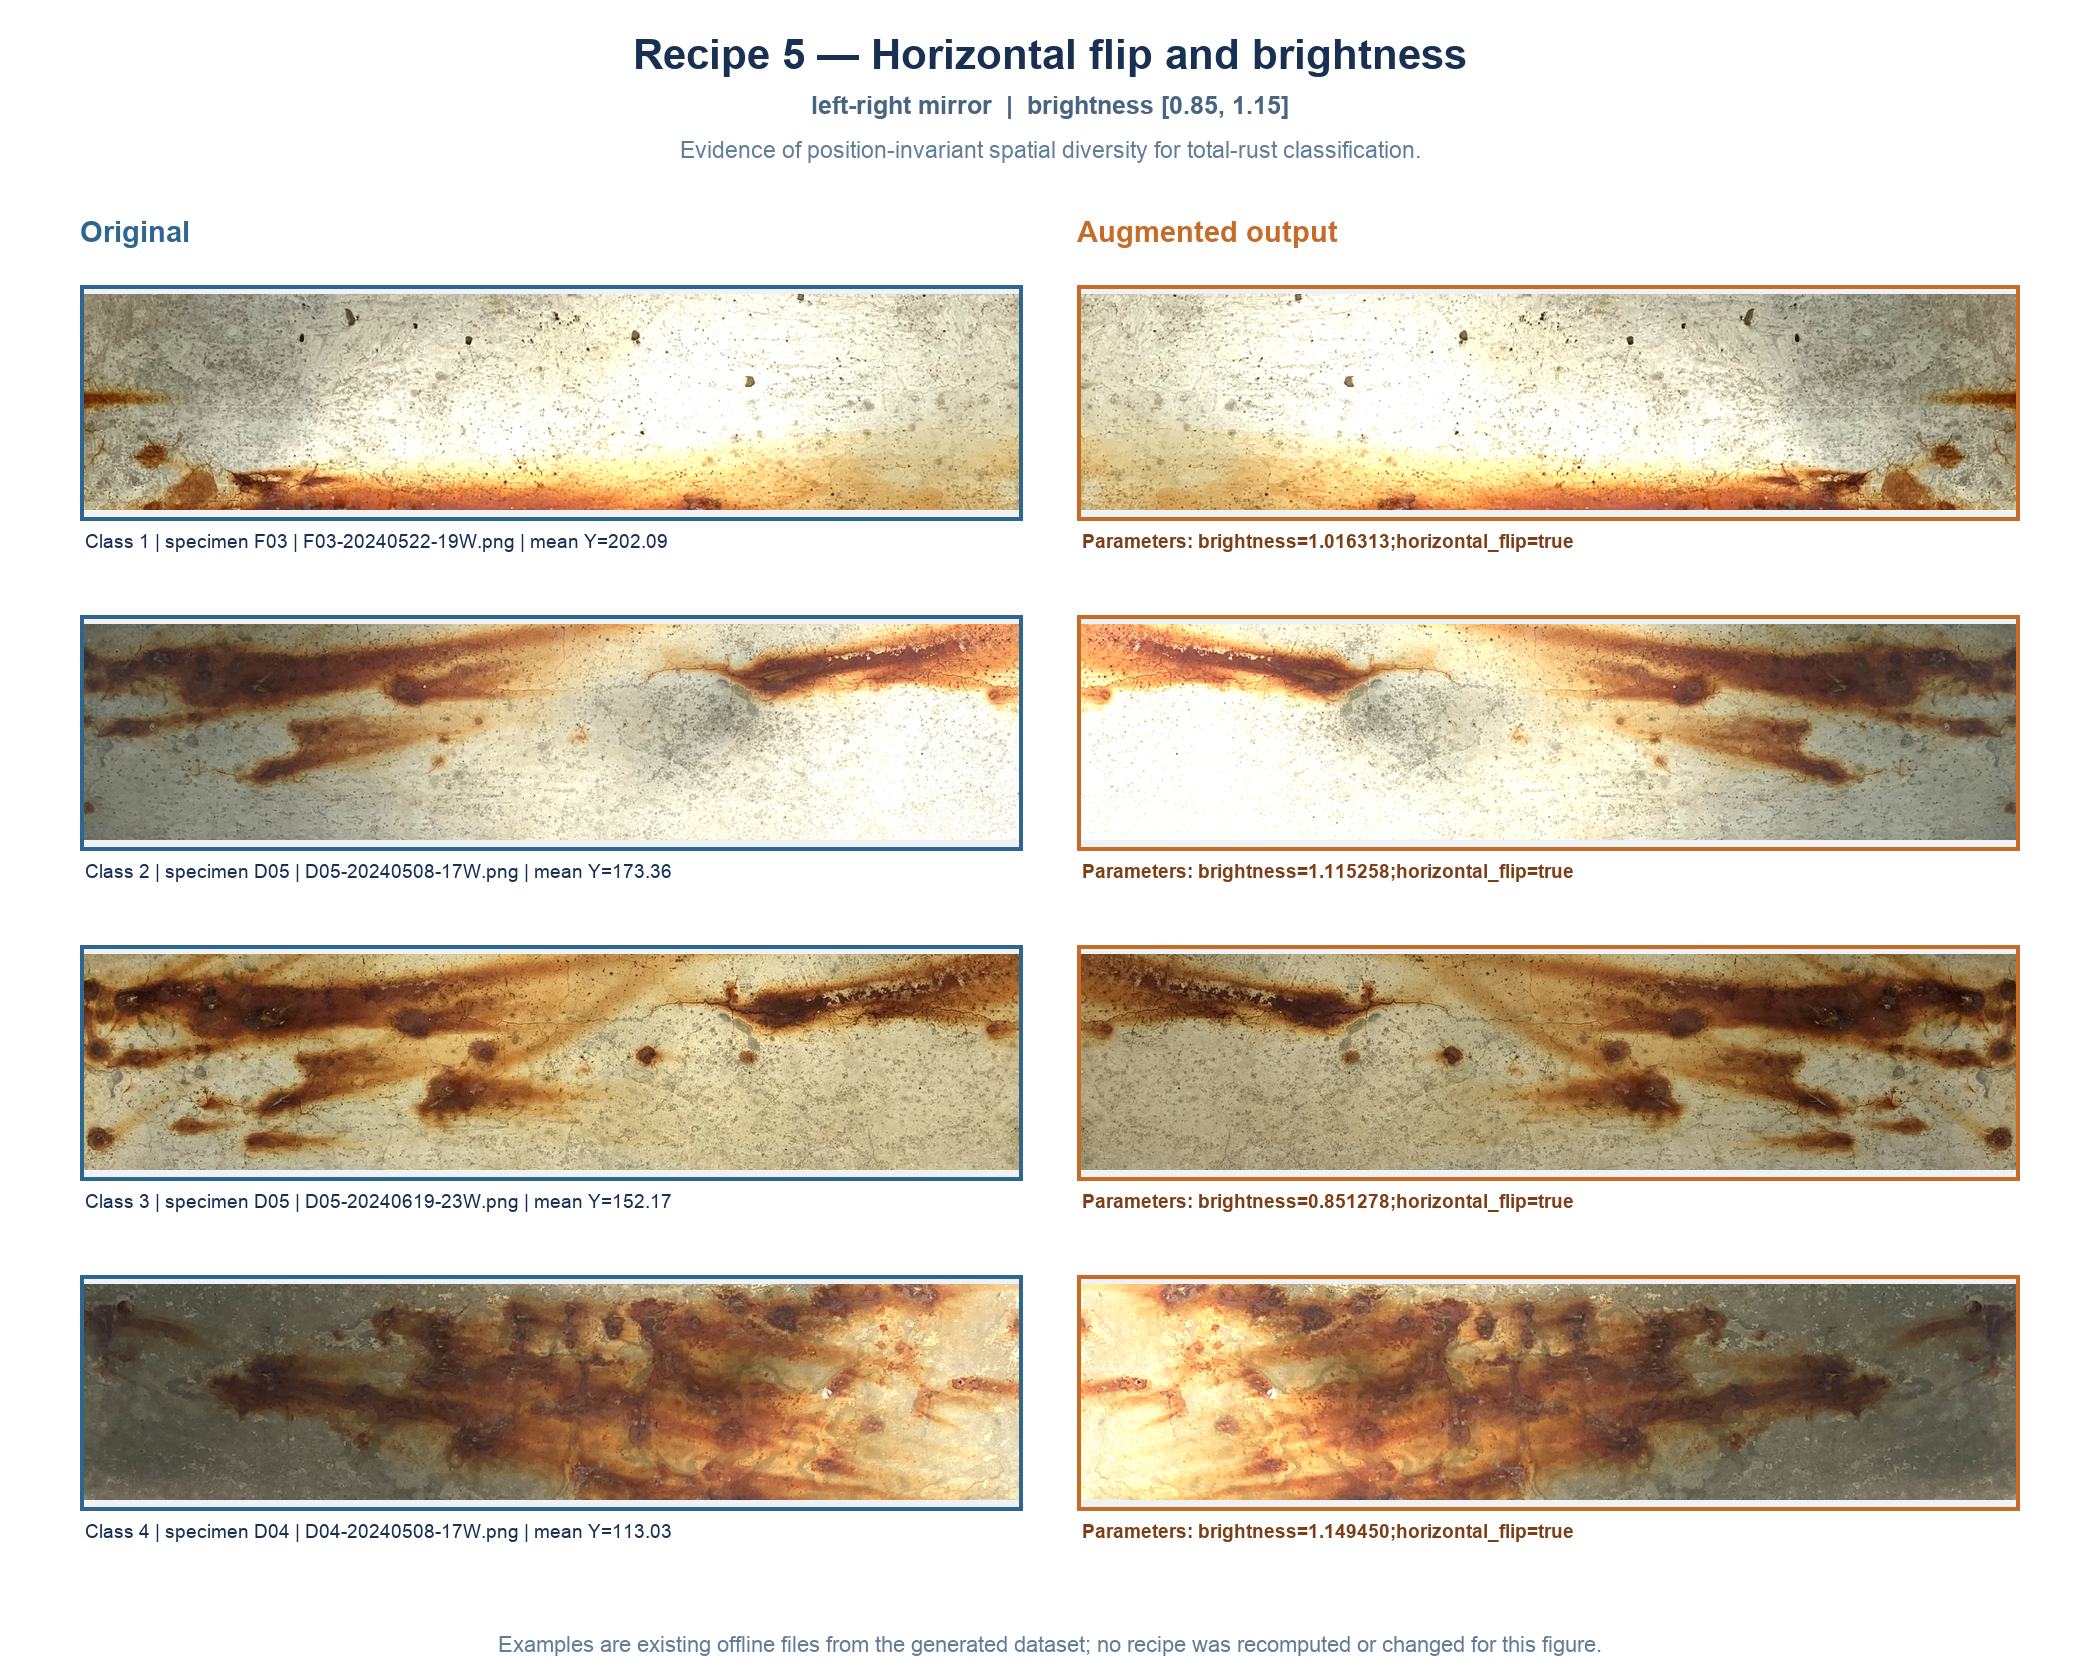
\includegraphics[width=\textwidth]{../augmentation/figures/recipe5_flip_brightness.png}
  \caption{Recipe~5 (left-right mirror and brightness): one original per class (left)
           and its mirrored-and-brightness-adjusted copy (right). The mirror effect
           is clearly visible; total rust coverage is unchanged.}
  \label{fig:recipe5}
\end{figure}

%% =============================================================================
\section{Rejected Augmentation Techniques}
\label{sec:rejected}
%% =============================================================================

Table~\ref{tab:rejected} lists techniques that were considered and explains why each was excluded.

\begin{longtable}{L{3.2cm} L{11.2cm}}
  \caption{Augmentation techniques considered and excluded.}
  \label{tab:rejected}\\
  \toprule
  \textbf{Technique} & \textbf{Reason for exclusion} \\
  \midrule
  \endfirsthead
  \multicolumn{2}{l}{\small\textit{Table~\ref{tab:rejected} continued from previous page}} \\[4pt]
  \toprule
  \textbf{Technique} & \textbf{Reason for exclusion} \\
  \midrule
  \endhead
  \bottomrule
  \endlastfoot

  MixUp
    & Blends two images together and adjusts the class label proportionally. The
      result---for example, ``60\% class~2 and 40\% class~3''---is not a
      physically meaningful rust severity. The four-class labels used in this
      study are discrete; they cannot be meaningfully interpolated. \\[6pt]

  CutMix
    & Pastes a rectangular patch from one image into another and adjusts the
      label proportionally to the pasted area. A patch of clean concrete pasted
      into a severe-rust image creates a contradictory training example: the
      label suggests moderate severity, but a region of the image shows no rust
      at all. For specimens in classes~2 and~3, where total rust coverage is
      already limited, this creates the largest risk of label corruption. \\[6pt]

  Synthetic image generation (GAN, diffusion)
    & Generating new corrosion images using a generative model would require
      training a separate model on fewer than 20 images per class for classes~3
      and~4. Models trained on so few examples produce unstable or repetitive
      outputs. This technique is not among the professor's specified families
      and is outside the scope of this study. \\[6pt]

  Elastic deformation
    & Warps the image as if the surface were made of elastic material. This
      technique was developed for medical imaging (deformable tissue in
      histology slides and MRI scans). A flat ferrocement slab photographed
      perpendicular to its surface does not deform in this way; applying
      elastic deformation produces physically implausible specimen images. \\[6pt]

  Random region removal (Cutout)
    & Replaces a random rectangular region of the image with black pixels. If
      the removed region contains the primary rust patch, the model receives an
      image labelled ``moderate rust'' that visually shows mostly clean
      concrete. For class~3 (20 images, limited rust coverage), this risk is
      highest. \\[6pt]

  Heavy colour shift ($>{}\pm10\%$)
    & Shifting the hue of the image by more than approximately 10--18$^\circ$
      on the colour circle can move rust pixels from their orange-red range into
      yellow, green, or magenta---colours that do not occur in corroded
      ferrocement. \\[6pt]

  Vertical mirror
    & Produces an upside-down photograph of the specimen. Not a plausible
      acquisition condition for this fixed imaging setup. \\[6pt]

  Large rotation ($>{}\pm10^\circ$)
    & Creates corner fill regions that are not representative of real specimen
      content. The imaging setup is fixed and does not produce rotated images.
\end{longtable}

%% =============================================================================
\section{Dataset Expansion Factor}
\label{sec:expansion}
%% =============================================================================

\subsection*{Resulting dataset}

Table~\ref{tab:expansion} shows the dataset size before and after augmentation.

\begin{table}[htbp]
  \centering
  \caption{Dataset size before and after augmentation.}
  \label{tab:expansion}
  \begin{tabular}{crrrc}
    \toprule
    \textbf{Class} & \textbf{Original images} & \textbf{Augmented copies}
      & \textbf{Total} & \textbf{Factor} \\
    \midrule
    1 &   658 &  3\,290 &  3\,948 & $6\times$ \\
    2 &    99 &    495  &    594  & $6\times$ \\
    3 &    20 &    100  &    120  & $6\times$ \\
    4 &    14 &     70  &     84  & $6\times$ \\
    \midrule
    \textbf{Total} & \textbf{791} & \textbf{3\,955} & \textbf{4\,746}
      & $\mathbf{6\times}$ \\
    \bottomrule
  \end{tabular}
\end{table}

\subsection*{Literature basis for the $6\times$ factor}

The expansion factor of $6\times$ (one original plus five augmented copies) was chosen to match the range supported by published corrosion studies of comparable dataset size. Table~\ref{tab:literature} lists the most relevant references.

\begin{table}[htbp]
  \centering
  \caption{Expansion factors in comparable published studies.}
  \label{tab:literature}
  \small
  \begin{tabular}{L{3.8cm}L{2.6cm}L{2.2cm}L{2.0cm}L{2.7cm}}
    \toprule
    \textbf{Study} & \textbf{Architecture} & \textbf{Dataset (pre-aug.)}
      & \textbf{Expansion} & \textbf{Result} \\
    \midrule
    Tank corrosion \cite{pmc11829104}
      & EfficientNetB0 & ${\sim}800$ images & $\mathbf{6.25\times}$ & \pct{94} accuracy \\
    Steel corrosion \cite{pmc11175235}
      & CNN & 100 images & $20\times$ & --- \\
    General survey \cite{shorten2019}
      & Various & Various & $\mathbf{2}$--$\mathbf{3\times}$ optimal & Diminishing returns above $3\times$ \\
    Steel defect detection
      & ResNet50, InceptionV3 & 800--2\,400 & $3\times$ & ${>}\pct{90}$ accuracy \\
    \bottomrule
  \end{tabular}
\end{table}

The most directly comparable study \cite{pmc11829104} (${\sim}800$ images, corrosion classification, offline augmentation) used $6.25\times$. The general survey \cite{shorten2019} identifies $2$--$3\times$ as optimal for larger datasets but acknowledges that corrosion-specific studies routinely use $3$--$6\times$ on smaller collections. The chosen $6\times$ sits at the upper boundary of this range.

\subsection*{Why $6\times$ was chosen over a higher factor}

Using each of the five recipes exactly once per source image gives $6\times$ and makes the composition of the training set transparent: every unique augmentation that the pipeline can produce appears exactly once. Generating more copies would require repeating recipes with different random parameters, introducing diminishing diversity per additional copy. No published corrosion study of comparable size justifies an expansion beyond 6--10$\times$, and the general survey \cite{shorten2019} reports minimal accuracy improvement above $3\times$. Six copies from five distinct recipe families is the natural stopping point.

%% =============================================================================
\section{Reproducibility}
\label{sec:repro}
%% =============================================================================

\subsection*{How the same augmented images are generated every time}

Every augmented image is produced using a random number that depends on three inputs: the global seed, the source image filename, and the copy number. These three inputs are combined using a standard cryptographic hash function (SHA-256), and the result is used to initialise the random number generator independently for each image-copy pair. Changing any one of the three inputs produces a completely different sequence of random numbers.

This means the output of the script is fully deterministic. Running the script again with the same global seed produces byte-identical images. Running it on a different computer or with different numbers of parallel processes produces the same result. The order in which images are processed does not affect the outcome.

\subsection*{Global seed}

The global seed used for all augmentation is \textbf{20260630}. This value was chosen to match the date of the dataset generation run and has no mathematical significance beyond uniqueness.

\subsection*{Reproduction command}

\begin{lstlisting}[language=bash]
python augmentation/augment_dataset.py --copies 5 --seed 20260630 --overwrite
\end{lstlisting}

\subsection*{Provenance fields in the CSV}

Every row in \file{Data/Images_Dataset_A-Z-1_augmented.csv} contains:
\begin{itemize}
  \item \texttt{original\_image\_name}: the source file this row was derived from
  \item \texttt{augmentation\_type}: the recipe name applied
  \item \texttt{augmentation\_parameters}: the exact numerical values used\\
        (for example, \texttt{brightness=0.874061;horizontal\_flip=true})
  \item \texttt{is\_augmented}: whether this row is an original or an augmented copy
  \item \texttt{specimen\_id}: the specimen identifier, required for
        leakage-safe train/test splitting
\end{itemize}

%% =============================================================================
\section{Splitting: Augmented Images Belong to the Training Partition Only}
\label{sec:splitting}
%% =============================================================================

Augmented images must not appear in the validation or test sets. The validation and test sets measure how well the model performs on images that look like real photographs. Augmented images do not look exactly like real photographs---they are intentionally altered. Including them in evaluation would measure performance on artificially varied images rather than on the real-world distribution.

More importantly, no augmented copy of a validation or test specimen may appear in the training set. Because augmented copies retain the visual identity of their source specimen (same rust pattern, same spatial layout, with only adjusted brightness or colour), placing a copy in training while the original is in the test set constitutes a data leak: the model has effectively seen the specimen before, in a slightly different form.

The split manifests produced by \file{augmentation/make_splits.py} implement these rules:
\begin{itemize}
  \item \textbf{Training rows:} all rows (original $+$ augmented) for the 38 training specimens.
  \item \textbf{Validation rows:} original rows only for 5 validation specimens.
  \item \textbf{Test rows:} original rows only for 5 test specimens.
  \item The 750 augmented copies of validation and test specimens are excluded from all splits.
\end{itemize}

%% =============================================================================
\section{Evidence Status Summary}
\label{sec:evidence}
%% =============================================================================

Table~\ref{tab:evidence} records the evidence basis and confidence level for every parameter choice in the pipeline.

\begin{table}[htbp]
  \centering
  \caption{Evidence basis for every parameter choice.}
  \label{tab:evidence}
  \small
  \begin{tabular}{L{2.6cm} L{2.4cm} L{6.7cm} L{2.5cm}}
    \toprule
    \textbf{Parameter} & \textbf{Value} & \textbf{Evidence basis} & \textbf{Confidence} \\
    \midrule
    Brightness lower bound  & 0.75
      & Measured: $1/(199.1/144.8) = 0.727 \to 0.75$
      & High \\[3pt]
    Brightness upper bound  & 1.28
      & Measured: $253.1/199.1 = 1.271 \to 1.28$
      & High \\[3pt]
    Contrast lower bound    & 0.78
      & Literature: industrial inspection $\pm15$--$25\%$
      & Medium \\[3pt]
    Contrast upper bound    & 1.25
      & Literature: industrial inspection $\pm15$--$25\%$
      & Medium \\[3pt]
    Colour intensity lower  & 0.78
      & Conservative heuristic; literature $\pm20$--$30\%$
      & Medium \\[3pt]
    Colour intensity upper  & 1.28
      & Conservative heuristic; literature $\pm20$--$30\%$
      & Medium \\[3pt]
    Colour shift per channel & $\pm6\%$ (0.94--1.06)
      & Measured: within-class $R/G$ std $\approx3\%$, range $\approx11\%$;
        chosen range covers this conservatively
      & Medium--high \\[3pt]
    Blur radius at source   & 0.3--1.5~px
      & Literature: industrial inspection 0.1--2.0~px
      & Medium \\[3pt]
    \textit{Blur at training res.} & \textit{0.12--0.59~px}
      & \textit{Derived from resize scale 0.394 (disclosure)}
      & \textit{High} \\[3pt]
    Noise level at source   & 0.005--0.035
      & Literature: surface inspection 0.01--0.05
      & Medium \\[3pt]
    \textit{Noise at training res.} & \textit{${\sim}0.003$--$0.022$}
      & \textit{Derived from resize scale (disclosure)}
      & \textit{High} \\[3pt]
    Combined recipe range   & 0.82--1.18
      & Engineering heuristic: $0.82^3 = 0.551$, keeps compound
        accumulation within ${\approx}50\%$
      & Medium \\[3pt]
    Mirror flip             & Fixed (no range)
      & Logical: total coverage is position-invariant
      & High \\[3pt]
    Flip brightness         & 0.85--1.15
      & Conservative sub-range of Recipe~1; heuristic
      & Low--medium \\[3pt]
    Expansion factor        & $6\times$
      & Literature: PMC11829104 ($6.25\times$); survey ($2$--$3\times$
        optimal for larger sets)
      & High \\[3pt]
    \bottomrule
  \end{tabular}
\end{table}

%% =============================================================================
\section{Limitations}
\label{sec:limitations}
%% =============================================================================

\paragraph{Contrast and colour intensity ranges are not measured from the dataset.}
The parameter ranges for light-to-dark contrast ($[0.78, 1.25]$) and colour intensity ($[0.78, 1.28]$) are drawn from published literature and set conservatively. A more rigorous calibration would measure the within-class variation in these properties and derive the range from that measurement, as was done for brightness. This analysis requires separating variation due to imaging conditions from variation due to physical specimen state (which correlates with the class label), and was not performed.

\paragraph{Blur is largely removed by downsampling.}
The blur applied at source resolution ($2835 \times 650$ pixels) is reduced to 0.12--0.59 effective pixels at training resolution ($224 \times 224$ pixels) by the resize operation during model training. The blurring contribution to model regularisation is therefore smaller than the stated source-resolution values suggest. Noise is similarly attenuated (to approximately 5.6~intensity units maximum at training resolution). Both effects are real and contribute to regularisation, but quantitatively less than the stated source-resolution values.

\paragraph{The class imbalance is preserved.}
Augmentation multiplies all classes by the same factor ($6\times$). Class~1 remains \pct{83.2} of the dataset. The model training must use class-weighted loss or an equivalent technique to address this imbalance.

\paragraph{The augmented dataset is fixed.}
Generating images offline means that only five specific random realisations of each recipe appear per source image. During model training, no new random variations are created per epoch. Online augmentation (applying transformations dynamically at training time) would produce greater variety at the cost of less convenient inspection and archiving. The offline approach was chosen for transparency and reproducibility.

%% =============================================================================
\section{Figures and Data Files}
\label{sec:files}
%% =============================================================================

Table~\ref{tab:files} lists all figure and data files produced by the augmentation pipeline.

\begin{table}[htbp]
  \centering
  \caption{Figures and data files produced by the augmentation pipeline.}
  \label{tab:files}
  \small
  \begin{tabular}{L{6.5cm} L{7.5cm}}
    \toprule
    \textbf{File} & \textbf{Content} \\
    \midrule
    \file{augmentation/figures/luminance_histogram.png}
      & Distribution of overall image brightness (all 791 images), with $p_5$~(144.8),
        median (197.7), and $p_{95}$~(253.1) marked. Shows the $1.75\times$ spread
        that motivates the brightness range. \\[4pt]
    \file{augmentation/figures/luminance_extremes.png}
      & Side-by-side of the four darkest images (specimen D04, class~4) and four
        brightest (G-series, class~1). Shows the full $2.60\times$ real-world
        variation. \\[4pt]
    \file{augmentation/figures/recipe1_brightness_contrast.png}
      & One original per class and its brightness-contrast augmented copy. \\[4pt]
    \file{augmentation/figures/recipe2_saturation_colour_balance.png}
      & One original per class and its colour-intensity-and-shift augmented copy. \\[4pt]
    \file{augmentation/figures/recipe3_blur_noise.png}
      & One original per class and its blur-and-noise augmented copy.
        Effect is intentionally subtle at source resolution. \\[4pt]
    \file{augmentation/figures/recipe4_combined.png}
      & One original per class and its combined-adjustment augmented copy. \\[4pt]
    \file{augmentation/figures/recipe5_flip_brightness.png}
      & One original per class and its mirrored-and-brightness-adjusted copy. \\[4pt]
    \file{augmentation/tables/image_statistics_full.csv}
      & Per-image statistics for all 791 source images: brightness, per-channel
        means, channel standard deviations, class label, specimen ID (791~rows). \\[4pt]
    \file{Data/Images_Dataset_A-Z-1_augmented.csv}
      & 4\,746-row provenance table: source filename, recipe, exact parameters,
        label, and specimen ID for every output image. \\
    \bottomrule
  \end{tabular}
\end{table}

\subsection*{Python library versions}

\begin{lstlisting}
Pillow   -- image loading, colour adjustment, blur, flip
NumPy    -- noise generation, array arithmetic
openpyxl -- Excel workbook reading
\end{lstlisting}

Exact installed versions are recorded in \file{augmentation/requirements.txt}.

%% =============================================================================
%% Bibliography
%% =============================================================================

\clearpage
\begin{thebibliography}{9}

\bibitem{touvron2021}
H.~Touvron, M.~Cord, M.~Douze, F.~Massa, A.~Sablayrolles, and H.~J\'{e}gou,
``Training data-efficient image transformers \& distillation through attention,''
in \textit{Proc.\ 38th Int.\ Conf.\ Machine Learning (ICML~2021)}, vol.~139,
pp.~10347--10357, 2021.

\bibitem{pmc11829104}
[Authors to be confirmed],
``Corrosion severity classification of storage tanks using deep learning
and offline data augmentation,''
\textit{[Journal --- placeholder]}, 2024.
PubMed Central~ID: PMC11829104.

\bibitem{pmc11175235}
[Authors to be confirmed],
``Automated steel corrosion classification using convolutional neural
networks with augmented training data,''
\textit{[Journal --- placeholder]}, 2024.
PubMed Central~ID: PMC11175235.

\bibitem{shorten2019}
C.~Shorten and T.~M.~Khoshgoftaar,
``A survey on image data augmentation for deep learning,''
\textit{Journal of Big Data}, vol.~6, no.~1, p.~60, 2019.
\href{https://doi.org/10.1186/s40537-019-0197-0}%
     {\texttt{doi:10.1186/s40537-019-0197-0}}
(arXiv:1906.11887).

\end{thebibliography}

\end{document}
